This chapter describes the development of $\pod$ $\numu$ and $\antinumu$
charged current (CC) inclusive\footnote{A CC-inclusive selection is a set of criteria that select all CC neutrino
interaction events as opposed to an CC-exclusive selection like CC-$0\pi$.} selections in both FHC and RHC beam configurations for the BANFF
fit. These selections are in continuation of previous works that developed
$\numu$ CC-inclusive selections between the $\pod$ and the TPC.
The first such analysis was the $\numu$ CC-inclusive cross section
using the previous ND280 simulation and reconstruction software release
called ``Production 5''\footnote{The ND280 detector reconstruction and Monte Carlo official software
updates are given a ``Production'' designation. The Production 5
software was actively used between 2012 and early 2014 until it was
replaced by Production 6. However, physics analyzers are not as rapid
to adopt the software updates.}\cite{Das2016}. That analysis relied on each subdetector's reconstruction
software and developed a track matching algorithm since the ND280
``Global'' reconstruction matching was not available in that software
production. Another cross section analysis measuring the cross section
ratio of $\numubar/\numu$ also used this ``pre-Global'' technique
with the modern ND280 ``Production 6'' software\footnote{The ND280 ``Production 6'' software was released in 2014 and is
still in active use.}\cite{AbePhyRevD9652017}. As the inter-detector matching reconstruction
became available in Global, two cross section analyzes, $\numu$ CC-$0\pi$\cite{PhysRevD.97.012001}
and $\numubar$ CC-$0\pi$\cite{AbeForthcoming,Campbell2018a}, were
developed that also used the CC-inclusive selection as pre-selection
cuts. A ``cut'' refers to one or more criteria to select reconstructed
events that have desired properties. The pre-selection cuts are designed
in particular to filter out poor data quality events. They are well
validated with results using these cuts are published as shown in
\prettyref{fig:numuandnumubarCC0pi}. The selections described in
this technote also employ the same pre-selection cuts with the latest
stable Global reconstruction software, Production 6.

\begin{figure}[t]
\begin{centering}
\subfloat[$\protect\numu$ CC-0$\pi$ Selection\cite{PhysRevD.97.012001}]{\begin{centering}
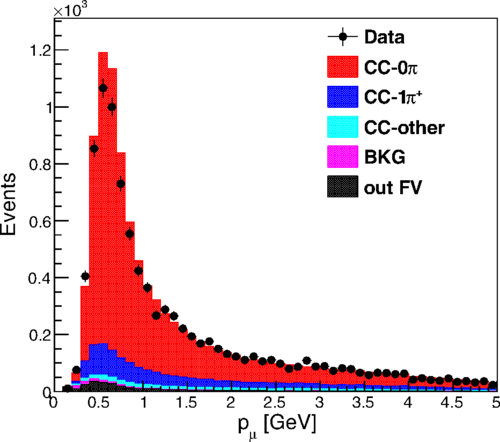
\includegraphics[height=0.25\textheight]{Chapters/Figures/SamplesAndSelections/cc0pi_selection}
\par\end{centering}
}\subfloat[$\protect\numubar$ CC-0$\pi$ Selection\cite{Campbell2018a}]{\begin{centering}
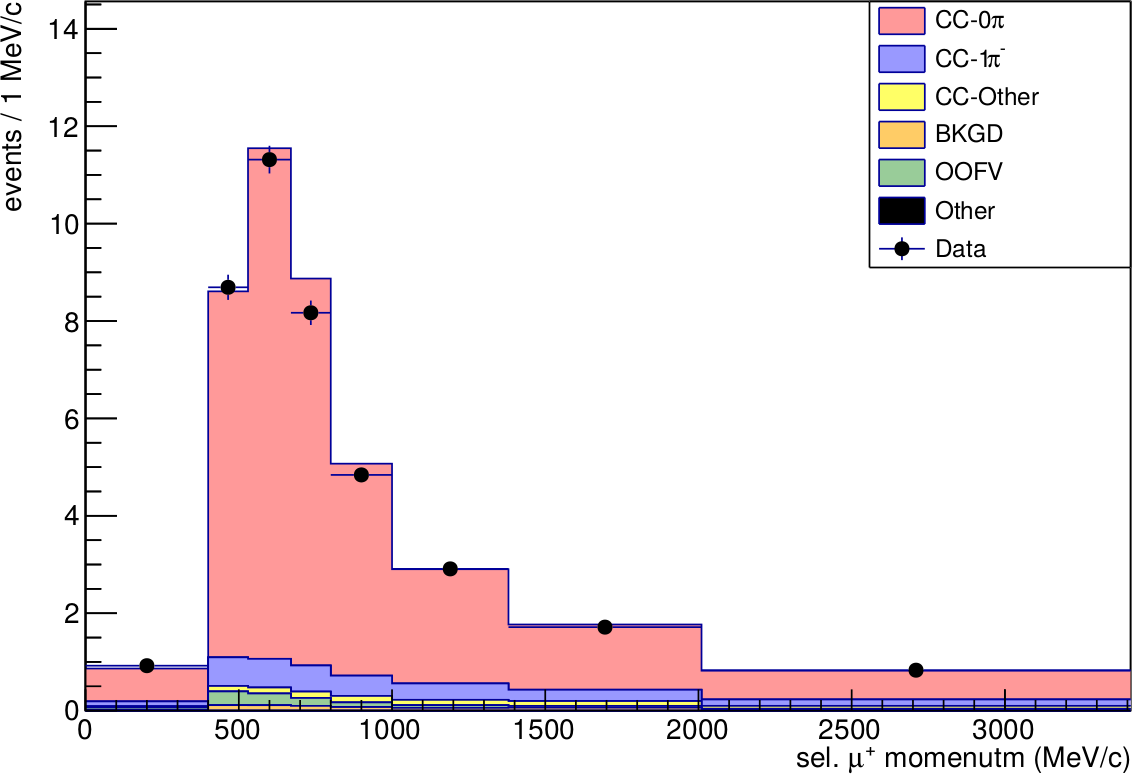
\includegraphics[height=0.25\textheight]{Chapters/Figures/SamplesAndSelections/numubarcc0pi_selection}
\par\end{centering}
}
\par\end{centering}
\caption[The \podtitle{} \numutitle{} and \numubartitle{} CC-$0\pi$ Selection
Kinematics]{The $\pod$ $\protect\numu$ and $\protect\numubar$ CC-$0\pi$ selection
kinematics. They importantly share the same pre-selection cuts as
this analysis. The error bars are statistical only with the prediction
sorted into various truth topologies.\label{fig:numuandnumubarCC0pi}}
\end{figure}

This paragraph is a layout of the topics in the chapter. First discussed
is the event reconstruction using the ``Global'' reconstruction
software in \prettyref{sec:The-ND280-Global-Reco}. The next discussion
is on the sample selections in \prettyref{sec:The-P0D-Selection-Cuts}.
With the selections established, three CC-inclusive selection are
described in the following order: the $\numu$ in foreword horn current
(FHC) mode selection, the $\numubar$ in reverse horn current (RHC)
mode selection, and the $\numu$ background in RHC mode selection.
The penultimate topic is an examination of the collected samples and
their kinematic properties in \prettyref{sec:Selection-Kinematics}.
Finally, the chapter summary is provided in \prettyref{sec:SelectionSummary}.


\section{The ND280 Global Reconstruction\label{sec:The-ND280-Global-Reco}}

The task of the Global reconstruction is to combine all of the ND280
information into a combined reconstructed object. It was originally
designed to identify CC-$0\pi$ events in the Tracker, FGD+TPC, region
and has been extended to operate with all of ND280.

The Global reconstruction is a software package that attempts to recognize
patterns of deposited energy in ND280 and categorize it accordingly.
Particles that deposit energy in long, linear segments are categorized
as tracks. If multiple tracks originate from a common origin (vertex),
it is likely that a true neutrino interaction event occurred near
the reconstructed vertex. Particle cascade or shower reconstruction
in Global will not be discussed since they are not selected in this
technote.

Each subdetector reconstruction algorithm is run separately as the
seed to Global's track matching algorithms. This includes the $\pod$'s
track-finding algorithm, which defines a $\pod$ track as a linear
sequence of ``nodes'' with one node at each bar layer. Each node
represents the approximate position where the particle intersected
the bar layer. To facilitate inter-detector matching, Global attempts
to ``re-fit'' the $\pod$ track using a Kalman filter\cite{kalmanFilter}.
The re-fit procedure also corrects for particle energy loss as a function
of length and multiple scattering processes. A $\pod$ vertex, which
is the assumed location of the neutrino interaction, is then associated
with the re-fit track using another Kalman filter algorithm. Matching
tracks between the $\pod$ and the TPC is done automatically in the
ND280 Global fit.


\section[Selection Cuts]{The \podtitle{} Selection Cuts\label{sec:The-P0D-Selection-Cuts}}

The selection of CC-inclusive events uses a series of cuts to select
the muon track. Prior to any cuts and after the reconstruction, corrections
are applied first to both data and MC events to correct for well known
residual differences between them. This includes correcting the MC
flux prediction using the secondary beamline data and reconstruction
efficiency corrections. A complete list of the corrections applied
are given in the following reference\cite{Abe2015c}. The pre-selection
cuts (``precuts'') are then applied to extract events that start
in the $\pod$ water target (WT) fiducial volume (FV).

The following sections will describe the precuts common to all CC-inclusive
selections. The next section describes the specific selections and
their cuts to select the main track associated as the lepton candidate.
Finally the lepton candidate and event kinematics for all the samples
are described.

\subsection{Precuts\label{subsec:Precuts}}

The precuts were initially developed to select $\numu$ CC-inclusive
events using the $\pod$ and TPC subdetector reconstruction algorithms
separately\cite{AbePhyRevD9652017,Das2016}. They were then used with
the Global reconstruction software for the $\numu$ $\cczeropi$ selection
in the FHC beam configuration\cite{PhysRevD.97.012001}. All cuts
were implemented in psyche\cite{Soto2017} which is the software interface
that BANFF uses to select events.

Prior to the precuts, neutrino interaction data event must be collected
and reconstructed for each T2K beam spill. Each T2K beam spill has
eight bunches that are 58 ns long and temporally separated by 581
ns. When the beam spill occurs, the $\pod$'s Trip-T electronics are
triggered to collect data in preset integration cycles aligned with
the bunches. Each integration cycle is 480 ns long and is followed
by a 100 ns dead-time to prepare for the next cycle\cite{Das2016}.
The data collected in each cycle is used to reconstruct neutrino interaction
events using the ND280 subdetector and Global software packages.

Each reconstructed event must pass the following cuts before being
assigned to a selection:
\begin{enumerate}
\item The event has a ``good'' data quality flag.
\begin{itemize}
\item An event is rejected if any electronics element or subdetector in
ND280 is reported as ``bad'' during the corresponding bunch.
\end{itemize}
\item There is at least one (1) track reconstructed in the TPC.
\begin{itemize}
\item There are no restrictions on the number of tracks fully contained
in the $\pod$ or exiting into other subdetectors. 
\end{itemize}
\item The track in the TPC must have more than 18 nodes.
\begin{itemize}
\item The TPC reconstruction gathers the vertical and horizontal micromegas
that registered collected charge into clusters of ``hits''. Each
cluster's charge distribution is used to get a vertical (horizontal)
position that is more accurate than the individual readout micromegas.
A node is constructed out of each cluster with associated track state
information. The set of nodes are used to fit a helix shaped track.
\end{itemize}
\item The reconstructed vertex is within the $\pod$ WT FV.
\begin{itemize}
\item The $\pod$ FV is defined to include as much of the WT regions as
possible. Its X and Y borders are 25 cm away from the $\pod$ule edges
while the Z borders intersect the last and first half downstream $\pod$ule
in the upstream ECal and central ECal, respectively. The FV edges
are listed in \prettyref{tab:FVDef}. This volume, while used for
track-based analyzes in the past, was optimized for $\pizero$ and
$\nue$ analyses.
\end{itemize}
\item All tracks that enter the TPC pass the veto cut
\begin{itemize}
\item An event is rejected if any $\pod$ track enters the TPC from outside
the ``corridor'' volume. This cut was designed to eliminate broken
tracks when the pre-Global separate subdetector reconstruction was
used \cite{Campbell2014}. In practice, this cut ensures that Global
tracks entering the TPC are away from its X and Y edges. The corridor
definition is the same as defined in the $\numubar/\numu$ cross section
ratio analysis technical note\cite{Campbell2017} and shown in \prettyref{tab:FVDef}.
\end{itemize}
\end{enumerate}
\begin{table}[H]
\caption[The \podtitle{} Water Target Fiducial Volume and Veto Corridor Definitions]{The $\pod$ WT FV (left) and veto corridor volume (right) in the
ND280 coordinate system. The corridor spans from the 5th (8th) to
40th (80th) $\pod$ule (scintillator layer). All the units are given
in millimeters.\label{tab:FVDef}}

\centering{}%
\begin{tabular}{cc}
\toprule 
\multicolumn{1}{c}{$\pod$ WT FV} & \multicolumn{1}{c}{Corridor Volume}\tabularnewline
\midrule
\midrule 
$-836<X<764$ & $-988<X<910$\tabularnewline
$-871<Y<869$ & $-1020<Y<1010$\tabularnewline
$-2969<Z<-1264$ & $-3139<Z<-900$\tabularnewline
\bottomrule
\end{tabular}
\end{table}

After passing of all the precuts, a single, global track, which is
observed in the TPC, is assigned as the lepton candidate or ``main
track'' of a selected event. While the main track is different for
each selected event, the momentum reconstruction is the same. The
momentum of the main track, $P$, is sum of its measured momentum
in the TPC, $P_{\text{TPC}}$, with the estimate momentum lost in
the $\pod$, $\Delta P_{\pod}$
\begin{equation}
P=P_{\text{TPC}}+\Delta P_{\pod}.\label{eq:momentumP0D}
\end{equation}
The momentum lost in the $\pod$ is estimated by summing the total
momentum loss along the track path $\mathcal{C}$ 
\begin{equation}
\Delta P=\int_{\mathcal{C}}\left(\frac{dP}{dx}\right)dx,\label{eq:energyloss}
\end{equation}
where $dP/dx$ is the momentum loss function. The momentum loss function
is related to the energy loss function, $dE/dx$ via the chain rule
\begin{equation}
\begin{aligned}\frac{dE}{dx} & =\left(\frac{dE}{dP}\right)\left(\frac{dP}{dx}\right)\\
 & =\frac{d}{dP}\left(\sqrt{P^{2}c^{2}+m^{2}c^{4}}\right)\left(\frac{dP}{dx}\right)\\
 & =\left(\frac{Pc^{2}}{E}\right)\left(\frac{dP}{dx}\right)\\
 & =\beta c\left(\frac{dP}{dx}\right),
\end{aligned}
\label{eq:chainrule}
\end{equation}
where $\beta$ is the particle velocity as a ratio of the speed of
light $c$. Since the reconstructed track's path $\mathcal{C}$ is
not infinitesimally precise due to inherent detector resolution, we
must replace the integral with a sum and differential $dx\rightarrow\Delta x$.
We then arrive at the expression of the momentum loss estimate in
the $\pod$ as
\begin{equation}
\Delta P_{\pod}=\frac{1}{c}\sum_{t}\left[\left(\frac{dE}{dx}\right)\left(\frac{\Delta x}{\beta}\right)\right]_{t},\label{eq:momentumP0DFull}
\end{equation}
where $t$ is a discrete step in $x$ connecting the track nodes.
For most tracks entering the TPC, they will be highly relativistic
in the $\pod$ ($\beta\approx1$), and \eqref{eq:momentumP0DFull}
simplifies to 
\begin{equation}
\Delta P_{\pod}=\frac{1}{c}\sum_{t}\left[\left(\frac{dE}{dx}\right)\Delta x\right]_{t}.\label{eq:momentumP0DSimplified}
\end{equation}
The next sections describe the selection cuts, first in FHC mode and
then RHC mode.

\subsection{The \numutitle{} in FHC Mode CC-Inclusive Selection \label{subsec:numuCCInclusive}}

As discussed in \mbox{Section~\ref{subsec:Precuts}}, this selection
is the basis for the $\pod$ $\numu$ $\cczeropi$ analysis\cite{PhysRevD.97.012001}.
In FHC mode, the vast majority of neutrino interactions are $\numu$
CC events that produce an outgoing, negatively charged muon. If there
is no negatively charged track in the TPC, the event is likely not
a $\numu$-induced interaction. Therefore, the $\numu$ in FHC mode
CC-inclusive selection in FHC mode has one final cut after the precuts:
\begin{enumerate}
\item At least one negatively charged track is reconstructed in the TPC.
\begin{itemize}
\item An event is rejected if none of the TPC tracks have a reported negative
curvature.
\end{itemize}
\end{enumerate}
If the event passes this cut, the highest momentum negative (curvature)
track, or HMNT, is selected as the lepton candidate. This selection
and all subsequent selections are branched into two categories based
on the number of tracks counted in the $\pod$. If there is only one
$\pod$ track, and hence only one track in the TPC as required by
the precuts, the event is categorized as a ``$\numu$ in FHC Mode
CC 1-Track'' event. Otherwise, the event is categorized as a ``$\numu$
in FHC Mode CC N-Tracks'' event.

\subsection{The \numubartitle{} in RHC Mode CC-Inclusive Selection \label{subsec:numubarRHCCCInclusive}}

In RHC mode, the majority of the beam neutrinos are $\numubar$ since
the horn focuses negatively charged pions and deflects positively
charged pions. However, the $\numu$ background interaction rate in
RHC mode is larger than the $\numubar$ background in FHC mode. The
reason for this is two fold. Firstly, the antineutrino-nuclear scattering
cross section is suppressed by \textasciitilde 1/3 compared to the
neutrino-nuclear scattering cross section as explained in \mbox{Section~\ref{subsec:Neutrino-Scattering-with-Matter}}.
Secondly, the $\numu$ flux in RHC is relatively large due to the
excess of positively charged pions generated at the target. Therefore
there is a non-negligible ``wrong-sign'' background in RHC mode
that we need to reject.

Prior to this analysis, a $\numubar$ CC-$0\pi$ selection was developed
for the $\pod$\cite{Campbell2018a}. The $\numubar$ CC-$0\pi$ selection
is quite similar to the $\numu$ CC-inclusive selection in FHC mode,
but relied on the $\pod$ local reconstruction for a particle identification
cut. The $\pod$ local reconstruction is, however, unavailable in
the event selection software used in the BANFF fit called psyche.
So a new selection was developed specifically for this analysis to
select $\numubar$ interactions in RHC mode.

The $\numubar$ in RHC mode CC-inclusive selection uses the precuts
described in \mbox{Section~\ref{subsec:Precuts}} and the has two
cuts:
\begin{enumerate}
\item At least one positively charged track is reconstructed in the TPC.
\begin{itemize}
\item An event is rejected if none of the TPC tracks have a reported positive
curvature.
\end{itemize}
\item The highest momentum positive (curvature) track, or HMPT, must be
the highest momentum track.
\begin{itemize}
\item If the highest momentum track has negative curvature, then the event
is rejected.
\end{itemize}
\end{enumerate}
If the event passes these two cuts, the HMPT is the lepton candidate.
If there is only one $\pod$ track, the event is categorized as a
``$\numubar$ in RHC Mode CC 1-Track'' event. Otherwise, the event
is categorized as a ``$\numubar$ in RHC Mode CC N-Tracks'' event.

\subsection{The \numutitle{} in RHC Mode CC-Inclusive Selection \label{subsec:numuRHCCCInclusive}}

As explained in the previous subsection, the $\numu$ background interaction
rate in RHC mode is relatively large compared to the $\numubar$ interaction
rate. Having a measurement of this background is critical for the
oscillation analysis due to the small number of expected $\numubar\rightarrow\nuebar$
counts. To date, there is no $\pod$ measurement of $\numu$ background
in RHC mode, nor any $\pod$ selection to do so. So like the $\numubar$
CC-inclusive selection, a new $\pod$ selection was developed exclusively
for this analysis to select $\numu$ background events in RHC mode.

The $\numu$ background in RHC mode CC-inclusive selection uses the
precuts described in Subsection \ref{subsec:Precuts} and has two
cuts:
\begin{enumerate}
\item At least one negatively charged track is reconstructed in the TPC.
\begin{itemize}
\item An event is rejected if none of the TPC tracks have a reported negative
curvature.
\end{itemize}
\item The HMNT must be the highest momentum track.
\begin{itemize}
\item If the highest momentum track has positive curvature, then the event
is rejected.
\end{itemize}
\end{enumerate}
If the event passes these two cuts, the HMNT is the lepton candidate.
If there is only one $\pod$ track, the event is categorized as a
``$\numu$ Background in RHC Mode CC 1-Track'' event. Otherwise,
the event is categorized as a ``$\numu$ Background in RHC Mode CC
N-Tracks'' event.


\section{Selection Kinematics\label{sec:Selection-Kinematics}}

This section examines the kinematics for each of selections and their
respective branches while differentiating between water-in and water-out
mode. The data sets used in this analysis are runs 2-8 in both $\pod$
water-in and water-out (air) modes as shown in \prettyref{tab:T2K-MC-Data-POT}.
There will be no data events shown to prevent any potential analysis
biases. Simulated events will be arranged into various true categories
to study selection kinematics, efficiencies, and purities.

\begin{table}
\caption[T2K Data-Taking Periods and Collected POT Used in the Analysis]{T2K data-taking periods and collected POT used in the analysis. The
bottom four rows are the aggregated periods grouped by horn current
and $\pod$ status, which is how the data analysis is performed. Note
that the horns were run briefly at +205 kA for Run 3b when operations
resumed after 2011 T\={o}hoku earthquake.\label{tab:T2K-MC-Data-POT}}

\centering{}%
\begin{tabular}{ccccc}
\toprule 
Run & Horn & $\pod$ & Data POT & MC POT\tabularnewline
period & current {[}kA{]} & status & $\left(\times10^{20}\right)$ & $\left(\times10^{20}\right)$\tabularnewline
\midrule
\midrule 
2 & +250 & Water & 0.433934 & 12.0341\tabularnewline
 &  & Air & 0.359149 & 9.23937\tabularnewline
3b & +205 &  & 0.217273 & 4.47864\tabularnewline
3c & +250 &  & 1.36447 & 26.3227\tabularnewline
4 &  &  & 1.78271 & 34.996\tabularnewline
 &  & Water & 1.64277 & 34.9712\tabularnewline
5c & -250 &  & 0.43468 & 22.7766\tabularnewline
6b &  & Air & 1.28838 & 14.174\tabularnewline
6c &  &  & 0.505895 & 5.27562\tabularnewline
6d &  &  & 0.775302 & 6.884\tabularnewline
6e &  &  & 0.847902 & 8.59439\tabularnewline
7b &  & Water & 2.43682 & 33.7046\tabularnewline
8 & +250 &  & 1.58053 & 26.4664\tabularnewline
 &  & Air & 4.14897 & 36.0694\tabularnewline
Sand & +250 &  & - & 11.1988\tabularnewline
Sand & -250 &  & - & 12.9201\tabularnewline
\midrule
\midrule 
2, 3b, 3c, 4, 8 & FHC & Air & 7.872757 & 111.09\tabularnewline
2, 4, 8 &  & Water & 3.656589 & 73.47\tabularnewline
6b, 6c, 6d, 6e & RHC & Air & 3.382490 & 35.262\tabularnewline
5c, 7b &  & Water & 2.852340 & 54.53\tabularnewline
\bottomrule
\end{tabular}
\end{table}

True interactions for these selections are generally divided into
four classes:
\begin{itemize}
\item A neutrino-induced CCQE interaction ($\nu$ CCQE):
\begin{itemize}
\item Only NEUT generated neutrino-induced CCQE event at the interaction
vertex.
\end{itemize}
\item A neutrino-induced non-CCQE interaction ($\nu$ non-CCQE):
\begin{itemize}
\item Any NEUT generated neutrino-induced CC and NC event \textit{except}
neutrino-induced CCQE at the interaction vertex.
\end{itemize}
\item An antineutrino-induced CCQE interaction ($\overline{\nu}$ CCQE):
\begin{itemize}
\item Only NEUT generated antineutrino-induced CCQE event at the interaction
vertex.
\end{itemize}
\item An antineutrino-induced non-CCQE interaction ($\overline{\nu}$ non-CCQE):
\begin{itemize}
\item Any NEUT generated antineutrino-induced CC and NC event \textit{except}
antineutrino-induced CCQE at the interaction vertex.
\end{itemize}
\end{itemize}
These signal classes must occur in the $\pod$ WT FV in order to be
selected. The non-CCQE category can be further divided among the dominant
T2K CC and all NC interactions modes as enumerated in \prettyref{tab:NEUTReaction}.
An out of FV (OOFV) event is any true event that occurs in ND280,
but is falsely reconstructed in the $\pod$ FV. Another important
ND280 background are true neutrino and antineutrino CC interactions
occurring in the sand surrounding the ND280 pit with the muon track
falsely reconstructed in the FV. These events are referred to as ``sand
muon'' events and are accounted for accordingly. Since these categories
are used frequently in this chapter, the legends used in the histograms
are enlarged for the reader's convenience in \prettyref{fig:enlarged_legends}.

\begin{table}
\caption[Enumeration of NEUT Interaction Modes]{Enumeration of the NEUT interaction modes which are also used in
\prettyref{fig:enlarged_legends}. An arrow indicates a sequence of
integer steps from left to right of the arrow. \label{tab:NEUTReaction}}

\centering{}%
\begin{tabular}{clc}
\toprule 
\multicolumn{2}{c}{Interaction mode} & $\nu$ ($\antinu$) NEUT enumeration\tabularnewline
\midrule
\midrule 
\multicolumn{2}{c}{CCQE} & $1$ ($-1$)\tabularnewline
\midrule 
 & 2p2h & $2$ ($-2)$\tabularnewline
\cmidrule{2-3} \cmidrule{3-3} 
 & CC-$1\pi$ & $11\rightarrow16$ ($-11\rightarrow-16$)\tabularnewline
\cmidrule{2-3} \cmidrule{3-3} 
\multirow{2}{*}{non-CCQE} & CC-N$\pi$ & $21$ ($-21$)\tabularnewline
\cmidrule{2-3} \cmidrule{3-3} 
 & CC-DIS & $26$ ($-26$)\tabularnewline
\cmidrule{2-3} \cmidrule{3-3} 
 & CC-Other & $17,22,23$ ($-17,-22,-23$)\tabularnewline
\cmidrule{2-3} \cmidrule{3-3} 
 & NC & $31\rightarrow100$ ($-31\rightarrow-100$)\tabularnewline
\bottomrule
\end{tabular}
\end{table}

The ND280 MC uses the GEANT4 software toolkit \cite{Agostinelli:2002hh}
to simulate the passage of particles through matter. A GEANT4 particle
is assigned to a reconstructed track if it contributed the most to
the track's reconstructed hits. The most likely truth matched particles
include protons (p), both negatively and positively charged muons
($\mu^{\pm}$), pions ($\pi^{\pm})$, and electrons/positrons ($e^{\pm})$.
In addition, any electron and positron generated from pair production
are grouped together as ``$e^{\pm}/\gamma$''. Particles that do
not match any of these categories is labeled as ``other''.

\begin{figure}
\begin{centering}
\subfloat[CCQE and non-CCQE]{\begin{centering}
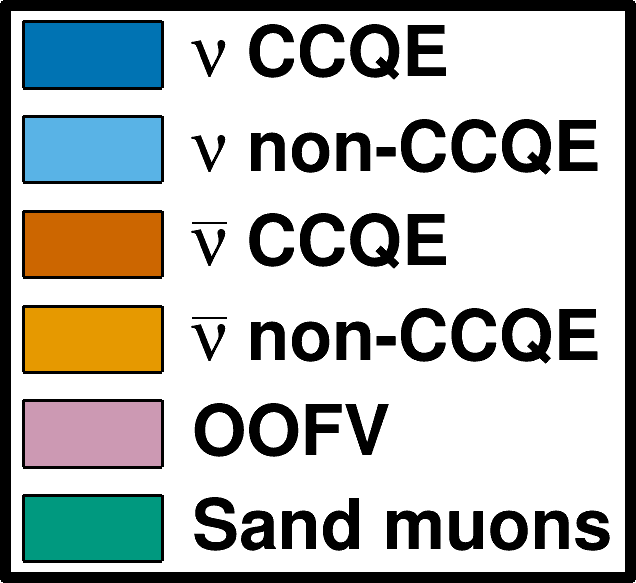
\includegraphics[height=1.32in]{Chapters/Figures/SamplesAndSelections/NEUTCCQELike_legend}
\par\end{centering}
}\subfloat[Neutrino interactions]{\begin{centering}
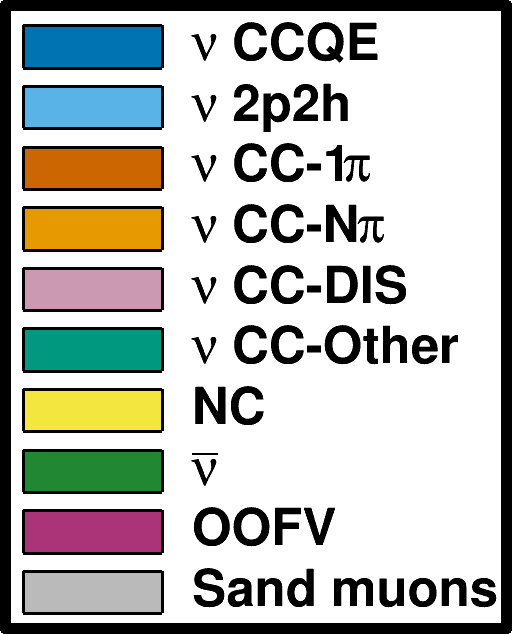
\includegraphics[height=2.26in]{Chapters/Figures/SamplesAndSelections/NEUTNuInteraction_legend}
\par\end{centering}
}\subfloat[Antineutrino interactions]{\centering{}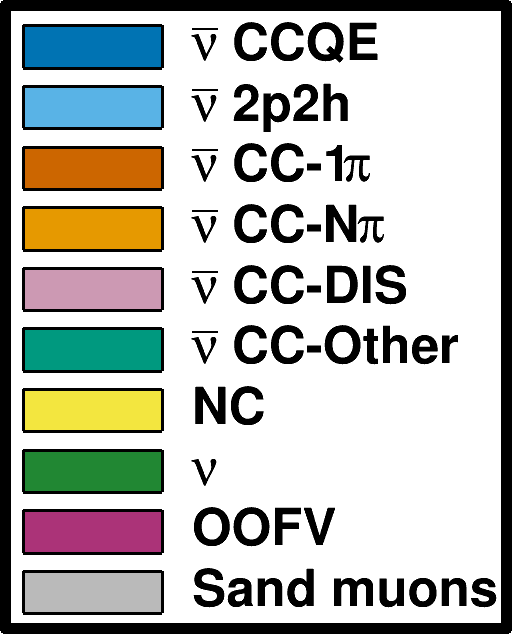
\includegraphics[height=2.26in]{Chapters/Figures/SamplesAndSelections/NEUTAntiNuInteraction_legend}}\subfloat[True particle]{\begin{centering}
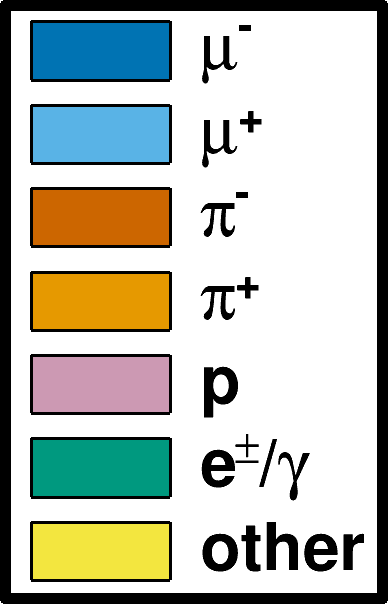
\includegraphics[height=1.57in]{Chapters/Figures/SamplesAndSelections/TrueParticle_legend}
\par\end{centering}
}
\par\end{centering}
\caption[Frequently Used Legends in the Analysis]{Frequently used legends that are enlarged for the reader's convenience.
\label{fig:enlarged_legends}}
\end{figure}


\subsection{The \numutitle{} in FHC Mode CC 1-Track Sample\label{subsec:numuFHCCC1Trk}}

This selection provides the CCQE-like samples in FHC mode. \prettyref{fig:numuFHCCC1TrkRecoCCQE}
and \prettyref{fig:numuFHCCC1TrkRecoParticle} displays the momentum
and angular distributions that are inputs to BANFF. Comparing between
water-in and water-out modes, we see that the reconstructed kinematics
are nearly identical. In the majority of cases, the lepton candidate
is the true muon, making this a very pure $\numu$ sample. We also
see that there are non-CCQE events, which without a particle identification
cut, are a irreducible background. Following this paragraph and the
following sections, only the $\pod$ water-in mode kinematics will
be shown.

\begin{figure}
\begin{centering}
\subfloat[Water-out Momentum]{\begin{centering}
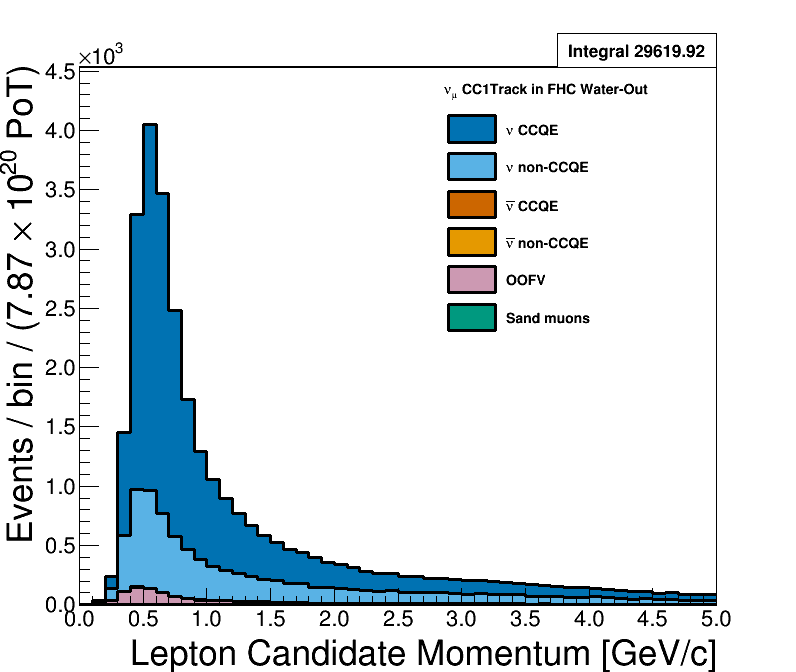
\includegraphics[width=0.45\textwidth]{Chapters/Figures/SamplesAndSelections/air/numu/CC1Track/FluxAndEventWeights/numuCC1TrackWaterOut_recoP_mu_MC_only_NEUTCCQELike_fhc_air}
\par\end{centering}
}\subfloat[Water-out $\cos\theta$]{\begin{centering}
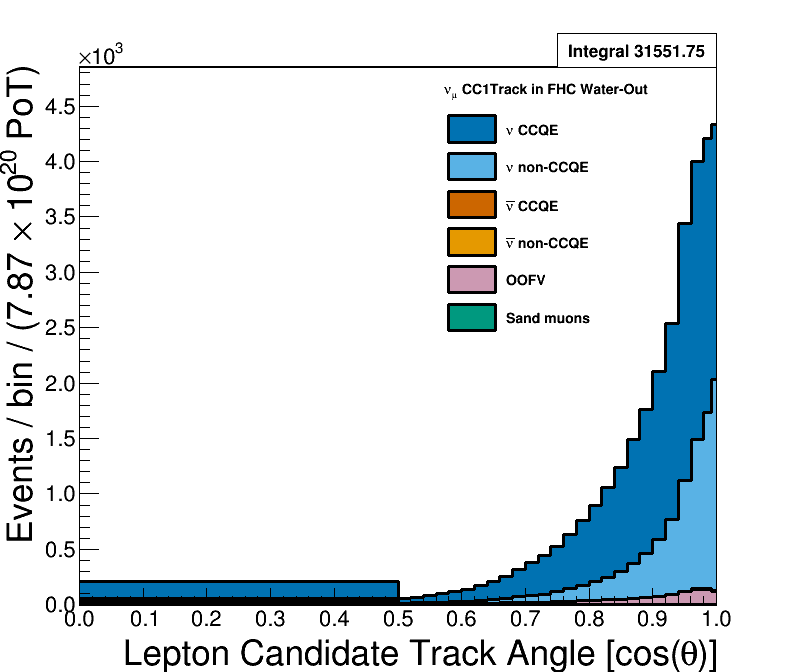
\includegraphics[width=0.45\textwidth]{Chapters/Figures/SamplesAndSelections/air/numu/CC1Track/FluxAndEventWeights/numuCC1TrackWaterOut_recocosq_mu_MC_only_NEUTCCQELike_fhc_air}
\par\end{centering}
}
\par\end{centering}
\begin{centering}
\subfloat[Water-in Momentum]{\begin{centering}
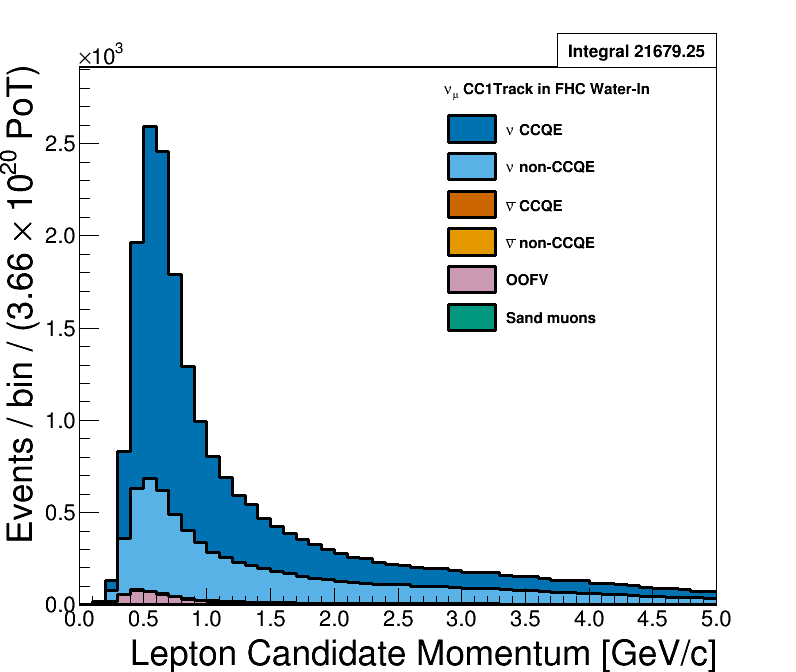
\includegraphics[width=0.45\textwidth]{Chapters/Figures/SamplesAndSelections/water/numu/CC1Track/FluxAndEventWeights/numuCC1TrackWaterIn_recoP_mu_MC_only_NEUTCCQELike_fhc_water}
\par\end{centering}
}\subfloat[Water-in $\cos\theta$]{\begin{centering}
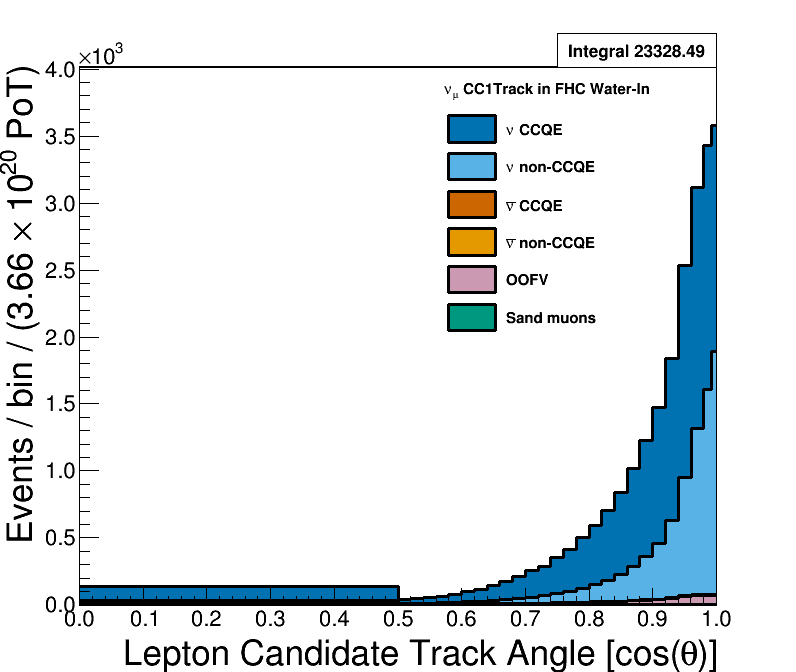
\includegraphics[width=0.45\textwidth]{Chapters/Figures/SamplesAndSelections/water/numu/CC1Track/FluxAndEventWeights/numuCC1TrackWaterIn_recocosq_mu_MC_only_NEUTCCQELike_fhc_water}
\par\end{centering}
}
\par\end{centering}
\caption[Reconstructed Kinematics of the $\numu$ in FHC Mode CC 1-Track Selection
Categorized by CCQE and Non-CCQE Interactions]{Reconstructed kinematics of the $\protect\numu$ in FHC Mode CC 1-Track
selection categorized by CCQE and non-CCQE interactions. The top figures,
(a) and (b), use the $\pod$ water-out MC and are normalized to the
FHC water-out mode POT. The bottom figures, (c) and (d), use the $\pod$
water-in MC and are normalized to the FHC water-in mode POT. Also
a single bin is used in the range of $0\protect\leq\cos\theta<0.5$
in figures (b) and (d).\label{fig:numuFHCCC1TrkRecoCCQE}}
\end{figure}

\begin{figure}
\begin{centering}
\subfloat[Water-out Momentum]{\begin{centering}
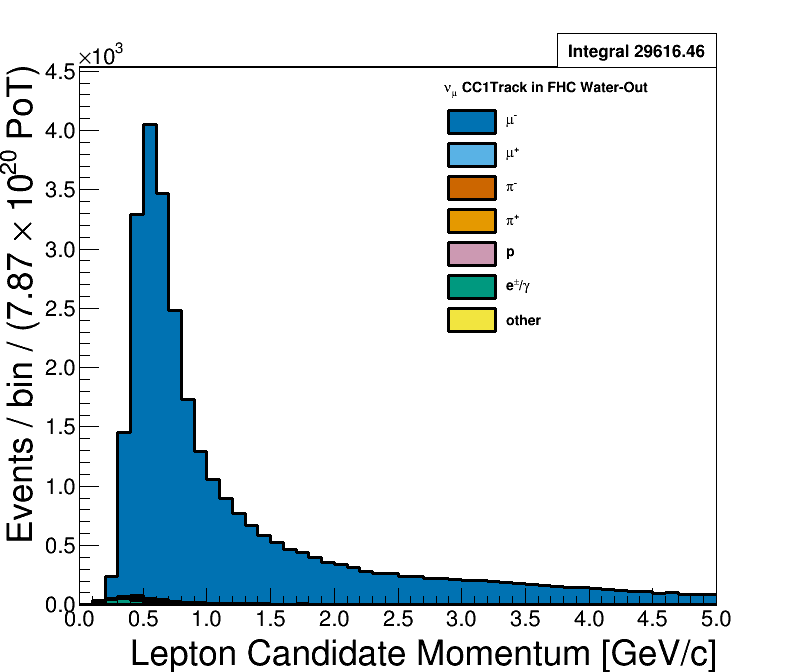
\includegraphics[width=0.45\textwidth]{Chapters/Figures/SamplesAndSelections/air/numu/CC1Track/FluxAndEventWeights/numuCC1TrackWaterOut_recoP_mu_MC_only_LeptonCandidateTruePDG_fhc_air}
\par\end{centering}
}\subfloat[Water-out $\cos\theta$]{\begin{centering}
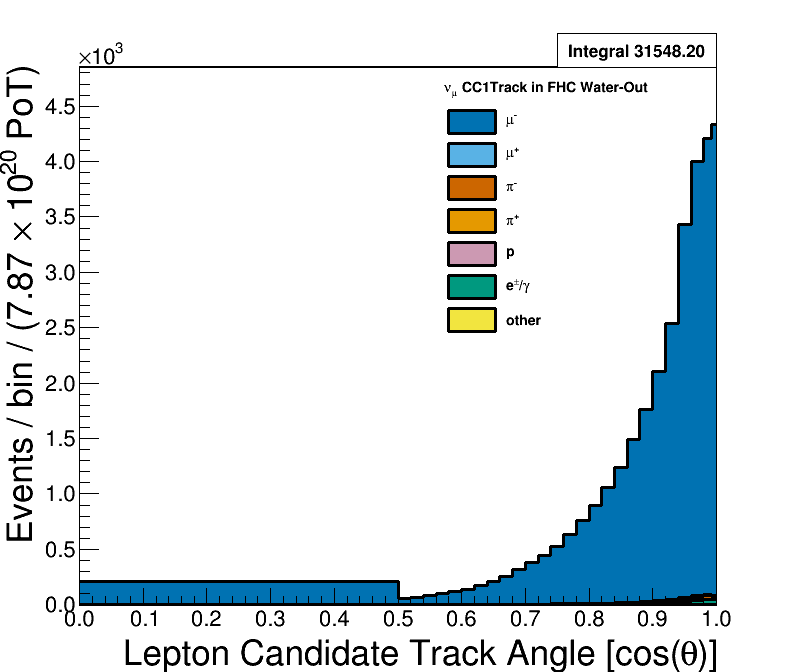
\includegraphics[width=0.45\textwidth]{Chapters/Figures/SamplesAndSelections/air/numu/CC1Track/FluxAndEventWeights/numuCC1TrackWaterOut_recocosq_mu_MC_only_LeptonCandidateTruePDG_fhc_air}
\par\end{centering}
}
\par\end{centering}
\begin{centering}
\subfloat[Water-in Momentum]{\begin{centering}
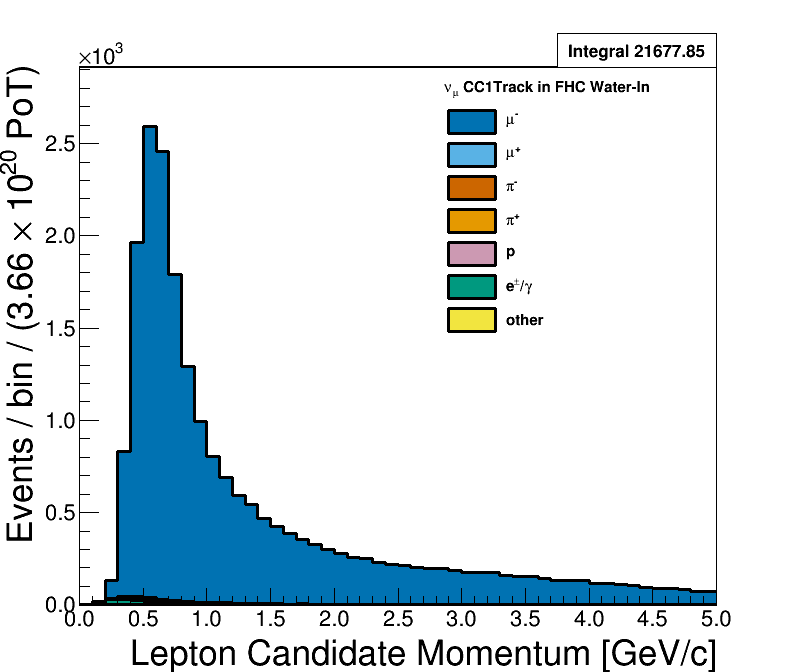
\includegraphics[width=0.45\textwidth]{Chapters/Figures/SamplesAndSelections/water/numu/CC1Track/FluxAndEventWeights/numuCC1TrackWaterIn_recoP_mu_MC_only_LeptonCandidateTruePDG_fhc_water}
\par\end{centering}
}\subfloat[Water-in $\cos\theta$]{\begin{centering}
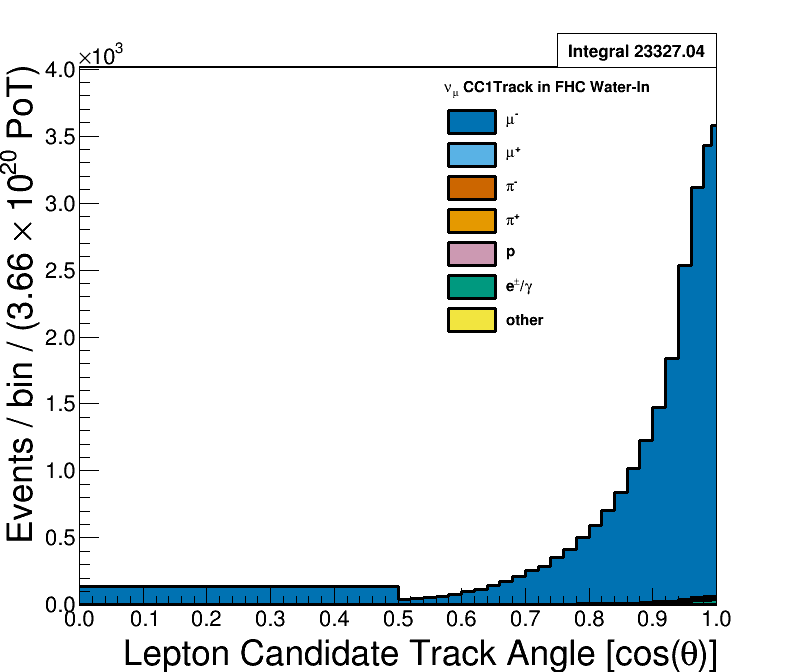
\includegraphics[width=0.45\textwidth]{Chapters/Figures/SamplesAndSelections/water/numu/CC1Track/FluxAndEventWeights/numuCC1TrackWaterIn_recocosq_mu_MC_only_LeptonCandidateTruePDG_fhc_water}
\par\end{centering}
}
\par\end{centering}
\caption[Reconstructed Kinematics of the $\numu$ in FHC Mode CC 1-Track Selection
Categorized by the True Particle Matched to the Main Track]{Reconstructed kinematics of the $\protect\numu$ in FHC Mode CC 1-Track
selection categorized by the true particle matched to the main track.
The top figures, (a) and (b), use the $\pod$ water-out MC and are
normalized to the FHC water-out mode POT. The bottom figures, (c)
and (d), use the $\pod$ water-in MC and are normalized to the FHC
water-in mode POT. Also a single bin is used in the range of $0\protect\leq\cos\theta<0.5$
in figures (b) and (d).\label{fig:numuFHCCC1TrkRecoParticle}}
\end{figure}

The target nuclei between water-in and water-out modes is shown in
\prettyref{fig:Vertex-position-numucc1trk}. Scattering on the carbon
nucleus is the dominant interaction in both modes since the scintillating
bars are constructed of polyethylene \ce{[(CH_2CH_2)_n]} plastic.
In water-in mode, the oxygen nucleus is a significant target with
hydrogen having a small contribution as well. The brass layers between
the $\pod$ules and the water bags introduce copper and zinc nuclei
scattering events too. The events on lead nuclei are true OOFV and
primarily occur in the last $\podule$.

\begin{figure}
\begin{centering}
\subfloat[Water-in]{\begin{centering}
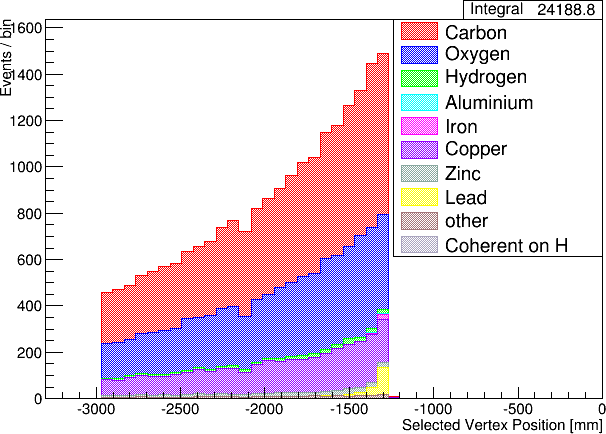
\includegraphics[width=0.45\textwidth]{Chapters/Figures/SamplesAndSelections/VertexZPosition_WaterIn_NumuFHCCC1Track}
\par\end{centering}
}\subfloat[Water-out]{\begin{centering}
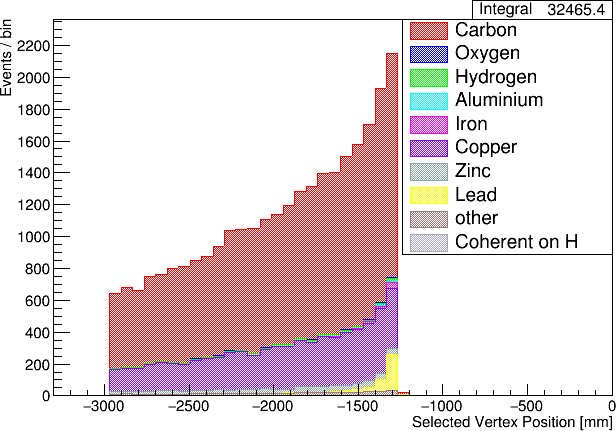
\includegraphics[width=0.45\textwidth]{Chapters/Figures/SamplesAndSelections/VertexZPosition_WaterOut_NumuFHCCC1Track}
\par\end{centering}
}
\par\end{centering}
\caption[Reconstructed Vertex Z Position of the $\numu$ in FHC Mode CC 1-Track
Selection]{Reconstructed vertex Z position of the $\protect\numu$ in FHC Mode
CC 1-Track selection. The events are categorized by the true target
nucleus. The number of selected events increases with increasing Z
since the probability of an interaction increases as the neutrino
crosses more media in the $\pod$. Due to a software bug in the MC,
coherent events on hydrogen (Coherent on H) are a unique category.\label{fig:Vertex-position-numucc1trk}}
\end{figure}

We can examine the efficiencies and purities differentially for true
$\numu$ CCQE interactions in \prettyref{fig:numuFHCCC1TrkRecoEffPur}.
The efficiency, $\epsilon$, and purity, $\rho$, are defined as
\begin{equation}
\epsilon=\frac{N_{\text{Selected}}^{\text{True}}}{N^{\text{True}}}\quad\rho=\frac{N_{\text{Selected}}^{\text{True}}}{N_{\text{Selected}}},\label{eq:effpur}
\end{equation}
where $N_{\text{Selected}}^{\text{True}}$ is the number of true,
selected events, $N^{\text{True}}$ is the number of true events,
and $N_{\text{Selected}}$ is the number of selected events. They
demonstrate that the purity is highest near $0.5$ GeV/c with the
efficiency highly dependent on the track angle.

\begin{figure}
\begin{centering}
\subfloat[True $\protect\numu$ CCQE Efficiency]{\begin{centering}
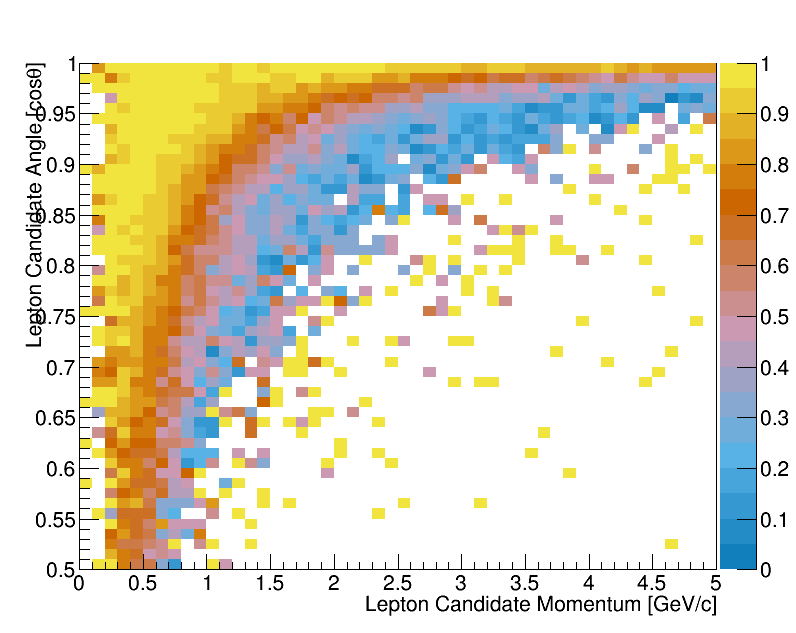
\includegraphics[width=0.45\textwidth]{Chapters/Figures/SamplesAndSelections/air/numu/CC1Track/FluxAndEventWeights/eff}
\par\end{centering}
}\subfloat[True $\protect\numu$ CCQE Purity]{\begin{centering}
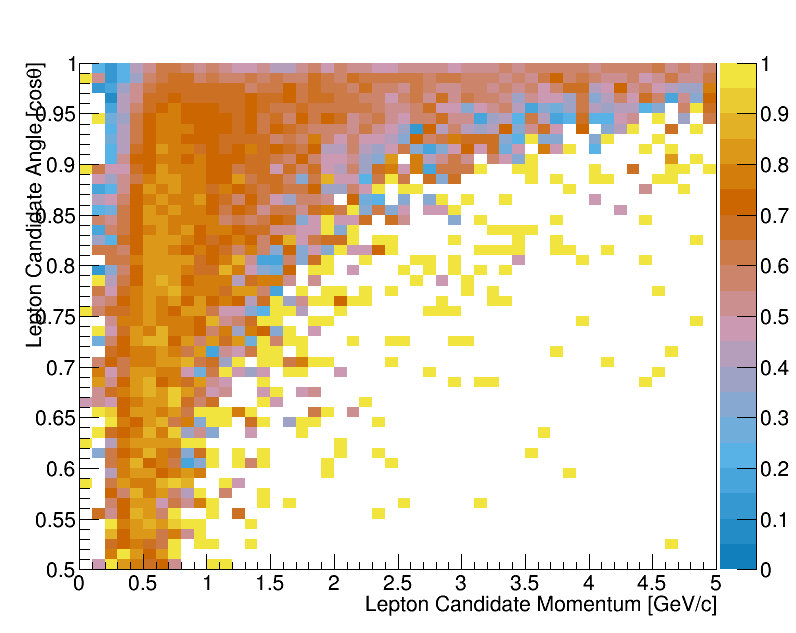
\includegraphics[width=0.45\textwidth]{Chapters/Figures/SamplesAndSelections/air/numu/CC1Track/FluxAndEventWeights/pur}
\par\end{centering}
}
\par\end{centering}
\caption[Efficiency and Purity of the $\numu$ in FHC Mode CC 1-Track Selection]{Efficiency and purity of the $\protect\numu$ in FHC Mode CC 1-Track
selection. True events are defined as correctly matched $\protect\muminus$
tracks from $\protect\numu$-induced CCQE interactions at the vertex.
\label{fig:numuFHCCC1TrkRecoEffPur}}
\end{figure}

The underlying true kinematics of the interactions are shown in \prettyref{fig:numuFHCCC1TrkTrue}.
Using \prettyref{fig:NuMuCCQE} as reference, the kinematics shown
are the true neutrino energy $E_{\nu}=k_{0}$ and 4-momentum transfer
$Q^{2}=-q^{2}$. These two variables are of theoretical importance
since they are used to generate events using NEUT and are used in
the BANFF fit. An interesting CCQE-like final state in this selection
are correlated nucleon pair scattering called ``2 particle, 2 hole''
(2p2h)\footnote{The name 2p2h originates from Condensed Matter Physics which motivated
the model. In solid state matter, a ``hole'' refers to the absence
of an electron in a valence band. In the High Energy Physics context,
2p2h considers neighboring and interacting nucleon pairs (2p) scattering
from an incoming neutrino. The imparted energy on the pair excites
them to higher energy states leaving two ``hole'' states (2h) behind.\medskip{}
} events\cite{Martini:2009uj}. Interaction model parameters for 2p2h
have large systematic uncertainties in T2K and are included the BANFF
fit. Therefore these events could help reduce the 2p2h model uncertainties.

\begin{figure}
\begin{centering}
\subfloat[True Neutrino Energy]{\begin{centering}
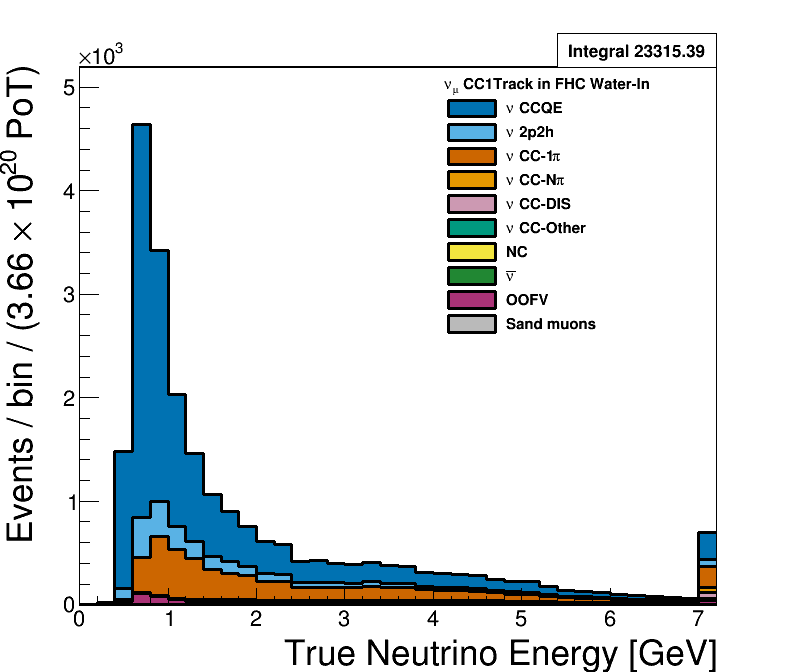
\includegraphics[width=0.45\textwidth]{Chapters/Figures/SamplesAndSelections/water/numu/CC1Track/FluxAndEventWeights/numuCC1TrackWaterIn_trueE_nu_MC_only_NEUTNuReactionCodes_fhc_water}
\par\end{centering}
}\subfloat[True $Q^{2}$]{\begin{centering}
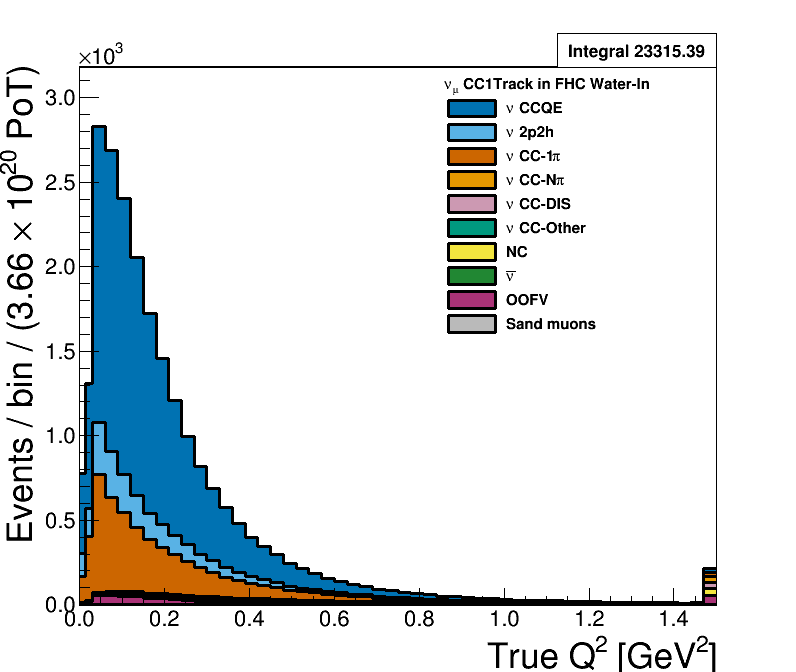
\includegraphics[width=0.45\textwidth]{Chapters/Figures/SamplesAndSelections/water/numu/CC1Track/FluxAndEventWeights/numuCC1TrackWaterIn_trueQ2_MC_only_NEUTNuReactionCodes_fhc_water}
\par\end{centering}
}
\par\end{centering}
\caption[True Kinematics of the $\numu$ in FHC Mode CC 1-Track Selection]{True kinematics of the $\protect\numu$ in FHC Mode CC 1-Track selection.
Water-in mode is displayed here only with the last bin shown is used
as overflow. The figures use the $\pod$ water-in MC and are normalized
to the FHC water-in mode POT. \label{fig:numuFHCCC1TrkTrue}}
\end{figure}

This selection contains a modest fraction of non-CCQE interactions.
The largest contamination is $1\pion$ interactions, which can happen
primarily for a couple of reasons. Firstly, when the final state pion
is produced, it is subject to final state interactions (FSI) where
a pion can be absorbed or scattered in the nucleus. Secondly, and
more importantly, a pion might not be reconstructed as a track in
the $\pod$ if its energy is below reconstruction threshold. Together,
the large $1\pion$ background affects the sensitivity to CC-$0\pi$
and CC-$1\pi$ model parameters in the BANFF fit.

\subsection{The \numutitle{} in FHC Mode CC N-Tracks Sample\label{subsec:numuFHCCCNTrk}}

This selection provides non-CCQE-like samples in FHC mode inputs to
the BANFF fit. The reconstructed momentum and angular distributions
are shown in \prettyref{fig:numuFHCCCNTrkRecoCCQE} and \prettyref{fig:numuFHCCCNTrkRecoParticle}.
Since this selection is not optimized for any particular CC topology,
there are a variety of interaction modes present including 1$\pion$,
multiple pion (N$\pion$) and deep inelastic scattering (DIS). There
are a number of events with a mis-identified main track that are matched
to electrons and pions. There is also a relatively larger OOFV contamination
compared with the 1-Track selection with some events originating in
the upstream ECal as seen in \prettyref{fig:Vertex-position-numuccNtrk}.
The vertex position and target materials are quite similar between
the 1-Track and N-Tracks selections.

\begin{figure}
\begin{centering}
\subfloat[Momentum]{\begin{centering}
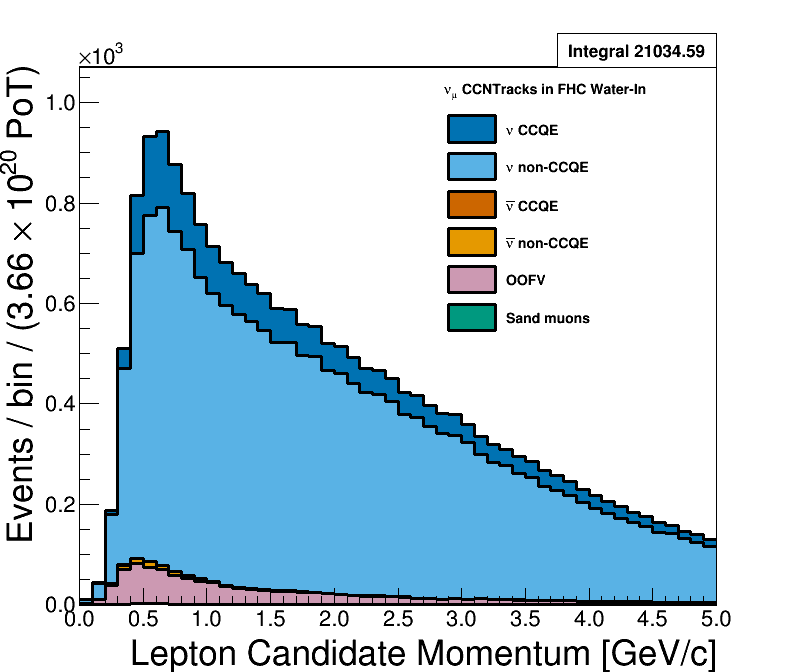
\includegraphics[width=0.45\textwidth]{Chapters/Figures/SamplesAndSelections/water/numu/CCNTracks/FluxAndEventWeights/numuCCNTracksWaterIn_recoP_mu_MC_only_NEUTCCQELike_fhc_water}
\par\end{centering}
}\subfloat[$\cos\theta$]{\begin{centering}
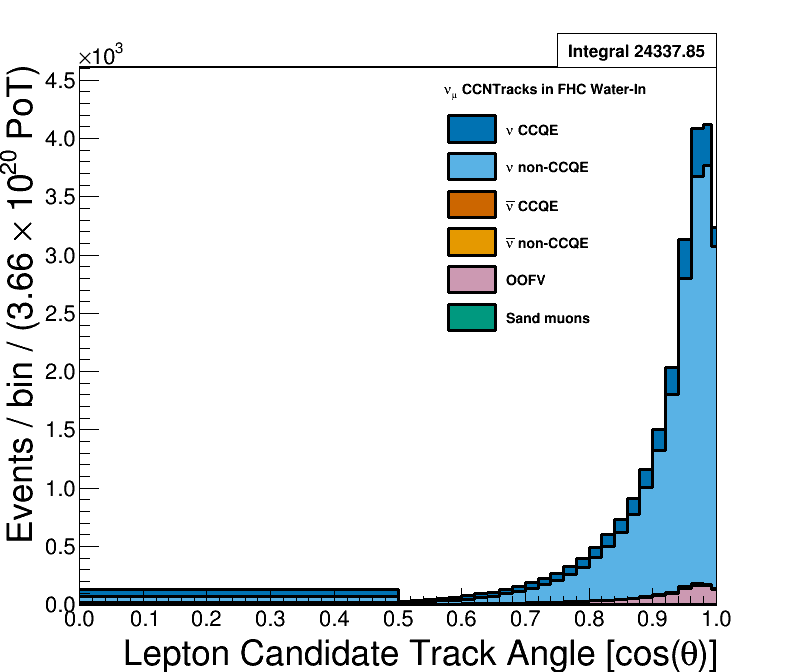
\includegraphics[width=0.45\textwidth]{Chapters/Figures/SamplesAndSelections/water/numu/CCNTracks/FluxAndEventWeights/numuCCNTracksWaterIn_recocosq_mu_MC_only_NEUTCCQELike_fhc_water}
\par\end{centering}
}
\par\end{centering}
\caption[Reconstructed Kinematics of the $\numu$ in FHC Mode CC N-Tracks Selection
Categorized by CCQE and Non-CCQE Interactions]{Reconstructed kinematics of the $\protect\numu$ in FHC Mode CC N-Tracks
selection categorized by CCQE and non-CCQE interactions. The figures
use the $\pod$ water-in MC and are normalized to the FHC water-in
mode POT. Also a single bin is used in the range of $0\protect\leq\cos\theta<0.5$
in figure (b).\label{fig:numuFHCCCNTrkRecoCCQE}}
\end{figure}

\begin{figure}
\begin{centering}
\subfloat[Momentum]{\begin{centering}
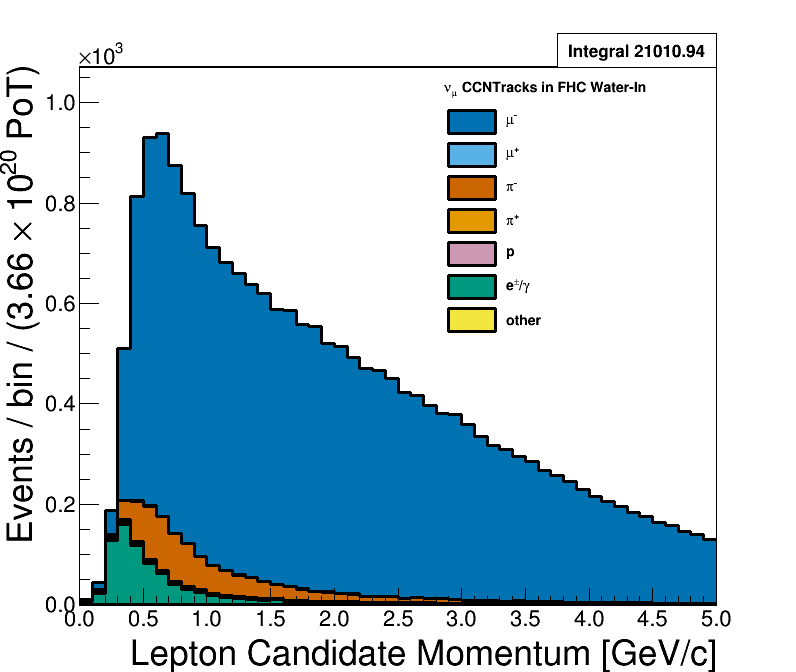
\includegraphics[width=0.45\textwidth]{Chapters/Figures/SamplesAndSelections/water/numu/CCNTracks/FluxAndEventWeights/numuCCNTracksWaterIn_recoP_mu_MC_only_LeptonCandidateTruePDG_fhc_water}
\par\end{centering}
}\subfloat[$\cos\theta$]{\begin{centering}
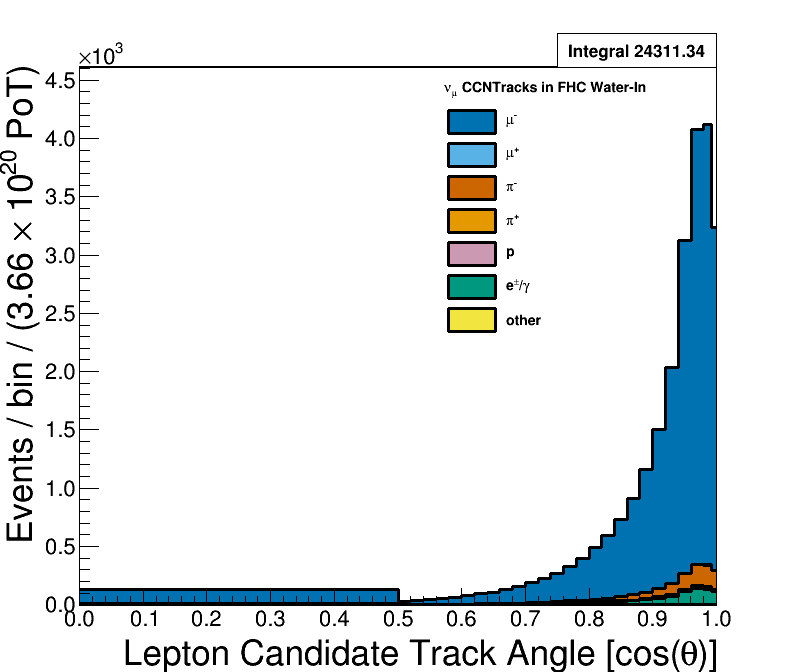
\includegraphics[width=0.45\textwidth]{Chapters/Figures/SamplesAndSelections/water/numu/CCNTracks/FluxAndEventWeights/numuCCNTracksWaterIn_recocosq_mu_MC_only_LeptonCandidateTruePDG_fhc_water}
\par\end{centering}
}
\par\end{centering}
\caption[Reconstructed Kinematics of the $\numu$ in FHC Mode CC N-Tracks Selection
Categorized by the True Particle Matched to the Main Track]{Reconstructed kinematics of the $\protect\numu$ in FHC Mode CC N-Tracks
selection categorized by the true particle matched to the main track.
The figures use the $\pod$ water-in MC and are normalized to the
FHC water-in mode POT. Also a single bin is used in the range of $0\protect\leq\cos\theta<0.5$
in figures (b) and (d).\label{fig:numuFHCCCNTrkRecoParticle}}
\end{figure}

\begin{figure}
\begin{centering}
\subfloat[Water-in]{\begin{centering}
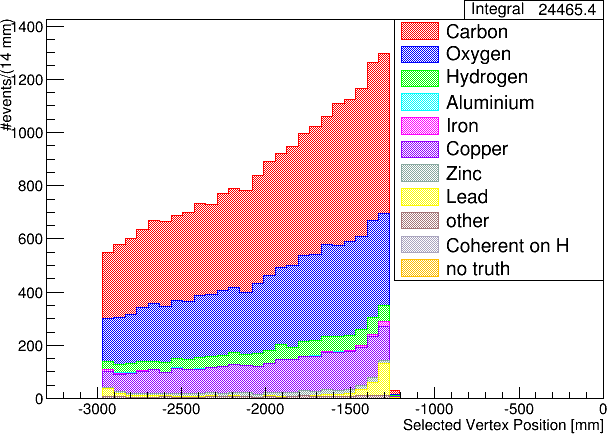
\includegraphics[width=0.45\textwidth]{Chapters/Figures/SamplesAndSelections/VertexZPosition_WaterIn_NumuFHCCCNTracks}
\par\end{centering}
}\subfloat[Water-out]{\begin{centering}
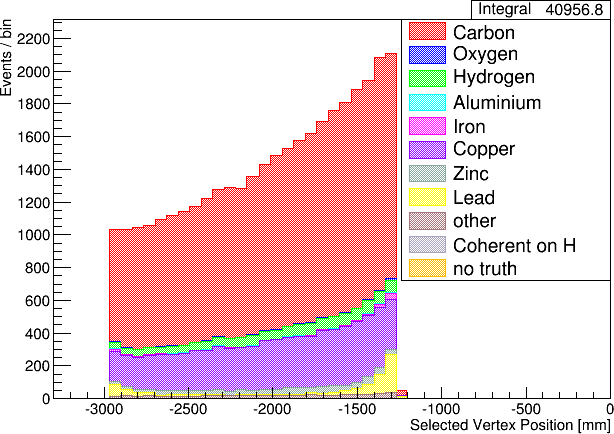
\includegraphics[width=0.45\textwidth]{Chapters/Figures/SamplesAndSelections/VertexZPosition_WaterOut_NumuFHCCCNTracks}
\par\end{centering}
}
\par\end{centering}
\caption[Reconstructed Vertex Z Position of the $\numu$ in FHC Mode CC N-Tracks
Selection Categorized by the True Target Nucleus]{Reconstructed vertex Z position of the $\protect\numu$ in FHC Mode
CC N-Tracks selection categorized by the true target nucleus. The
number of events increases with increasing Z since the probability
of an interaction increases as the neutrino crosses more media in
the $\pod$. Due to a software bug in the MC, coherent events on hydrogen
(Coherent on H) are a unique category.\label{fig:Vertex-position-numuccNtrk}}
\end{figure}

We can examine the efficiencies and purities differentially for the
selection in \prettyref{fig:numuFHCCCNTrkRecoEffPur}. For the efficiency
and purity only, the true signal is any $\numu$ CC interaction except
$\numu$ CCQE (CC non-QE), which the CC 1-Track topology selection
is designed to select. The efficiency is high for the higher momenta
and higher angle tracks suggesting this is a high $Q^{2}$ selection.
In addition, the purity is around \textasciitilde 70\% in this region.

\begin{figure}
\begin{centering}
\subfloat[True $\protect\numu$ CC non-QE Efficiency]{\begin{centering}
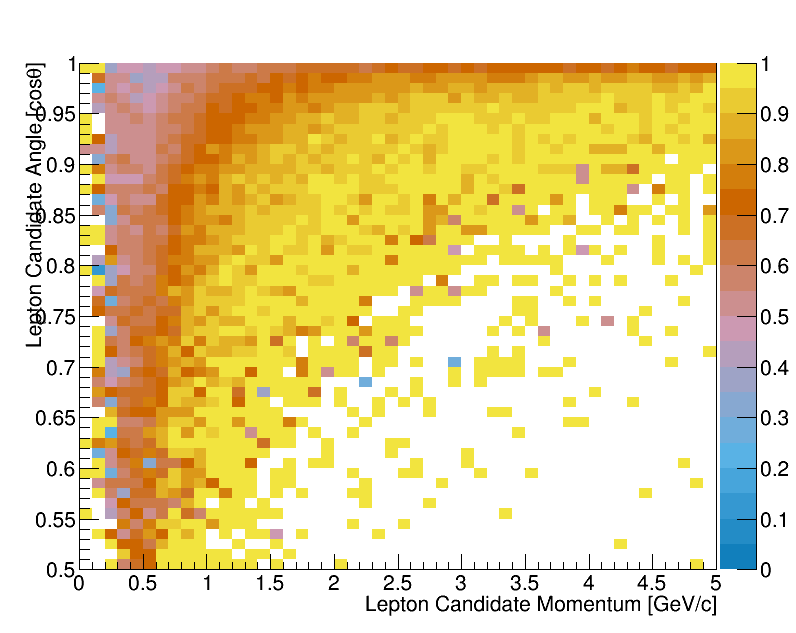
\includegraphics[width=0.45\textwidth]{Chapters/Figures/SamplesAndSelections/air/numu/CCNTracks/FluxAndEventWeights/eff}
\par\end{centering}
}\subfloat[True $\protect\numu$ CC non-QE Purity]{\begin{centering}
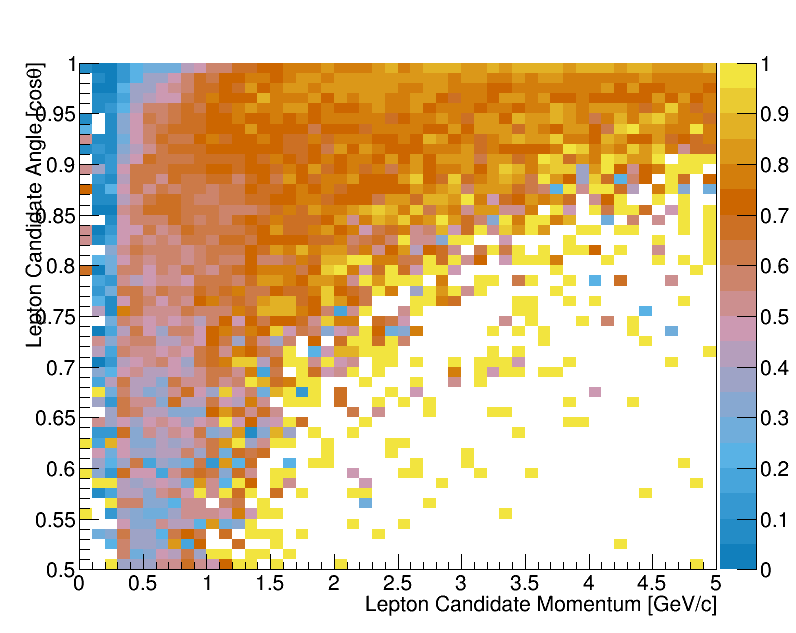
\includegraphics[width=0.45\textwidth]{Chapters/Figures/SamplesAndSelections/air/numu/CCNTracks/FluxAndEventWeights/pur}
\par\end{centering}
}
\par\end{centering}
\caption[Efficiency and Purity of the $\numu$ in FHC Mode CC N-Tracks Selection]{Efficiency and purity of the $\protect\numu$ in FHC Mode CC N-Tracks
selection. True events are defined as correctly matched $\protect\muminus$
tracks from $\protect\numu$-induced CC non-QE interactions at the
vertex.\label{fig:numuFHCCCNTrkRecoEffPur}}
\end{figure}

The fundamental kinematics of the selection are shown in \prettyref{fig:numuFHCCCNTrkTrue}.
The selection is relatively $\numu$-pure and captures the high energy
tail of the neutrino flux. True kinematics that describe the $1\pion,$
$N\pion$, and DIS models are parameterized in $Q^{2}$ and the hadronic
system mass $W$. Using \prettyref{fig:NuMuCCQE}, we can define the
invariant mass of hadronic system as
\begin{equation}
\begin{aligned}W^{2}c^{4} & =\left(p+q\right)^{2}=p^{2}+2p\cdot q+q^{2}\\
 & =M_{N}^{2}c^{4}+2M_{N}c^{2}\left(k_{0}-k_{0}^{\prime}\right)-Q^{2},
\end{aligned}
\label{eq:hadronicsystemmassW}
\end{equation}
where $M_{N}$ is the mass of the struck nucleon and $k_{0}$/$k_{0}^{\prime}$
is the energy of the neutrino/outgoing lepton. A dominant mode in
the selection is from the $1\pion$ interaction from a $\Delta$ resonance.
A resonance is clearly seen in the $W$ distribution in \prettyref{fig:numuFHCCCNTrkTrue},
which comes from the $\Delta$ baryon which has a rest mass of $1.232$
GeV/$\csq$.

\begin{figure}
\begin{centering}
\subfloat[True Neutrino Energy]{\begin{centering}
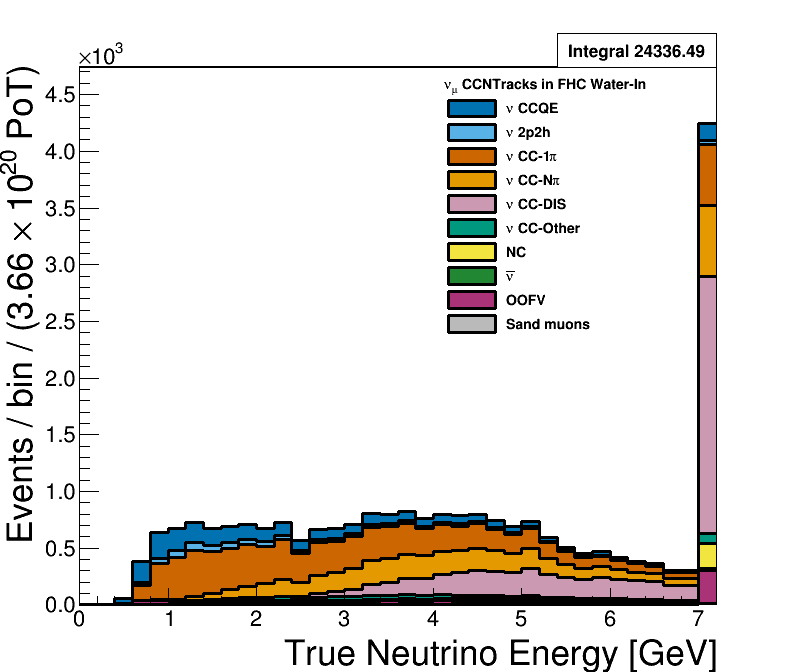
\includegraphics[width=0.45\textwidth]{Chapters/Figures/SamplesAndSelections/water/numu/CCNTracks/FluxAndEventWeights/numuCCNTracksWaterIn_trueE_nu_MC_only_NEUTNuReactionCodes_fhc_water}
\par\end{centering}
}\subfloat[True $Q^{2}$]{\begin{centering}
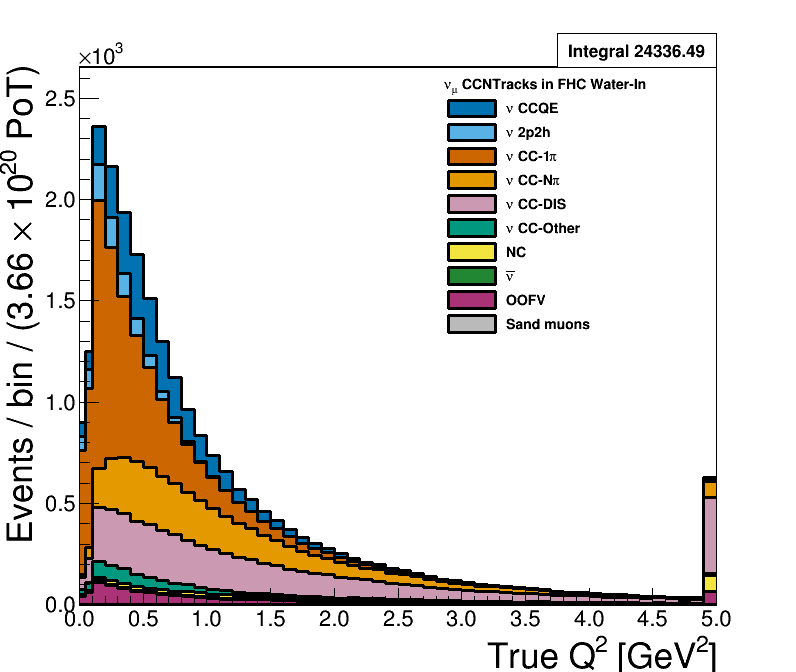
\includegraphics[width=0.45\textwidth]{Chapters/Figures/SamplesAndSelections/water/numu/CCNTracks/FluxAndEventWeights/numuCCNTracksWaterIn_trueQ2_MC_only_NEUTNuReactionCodes_fhc_water}
\par\end{centering}
}
\par\end{centering}
\begin{centering}
\subfloat[True $W$]{\begin{centering}
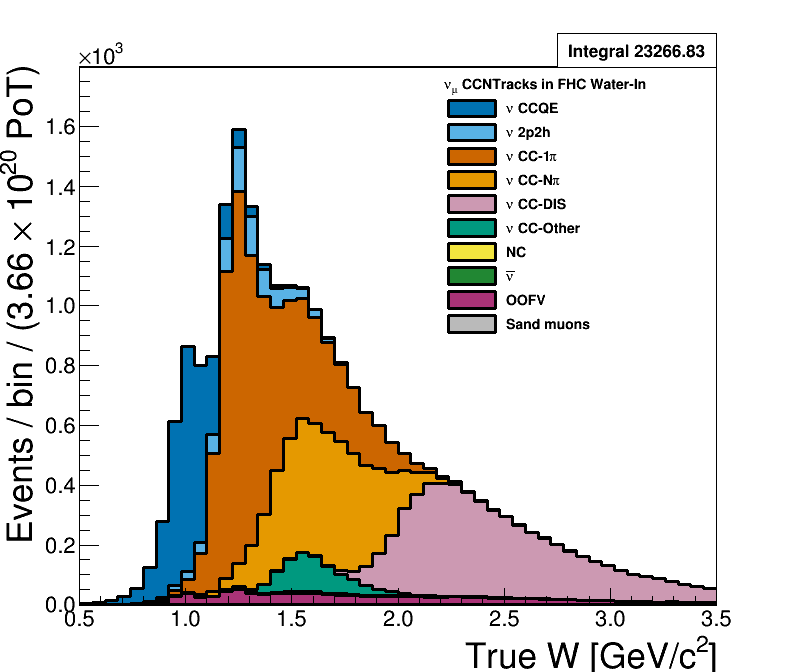
\includegraphics[width=0.45\textwidth]{Chapters/Figures/SamplesAndSelections/water/numu/CCNTracks/FluxAndEventWeights/numuCCNTracksWaterIn_trueW_MC_only_NEUTNuReactionCodes_fhc_water}
\par\end{centering}
}
\par\end{centering}
\caption[True Kinematics of the $\numu$ in FHC Mode CC N-Tracks Selection]{True kinematics of the $\protect\numu$ in FHC Mode CC N-Tracks selection.
The last bin shown in (a) and (b) is used as overflow. The figures
use the $\pod$ water-in MC and are normalized to the FHC water-in
mode POT. In figure (c), the largest resonance comes from the $\Delta$
baryon. There are higher order resonances in (c) as well.\label{fig:numuFHCCCNTrkTrue}}
\end{figure}

The origin of the mis-identified tracks, in particular the pion matched
tracks, becomes more clear since this is a high $Q^{2}$ selection.
The $N\pi$ and DIS events, which are high $Q^{2}$ events, can yield
a post-FSI charged pion track. These pions could have more energy
than the outgoing muon or could be the only particle observed in the
TPC.

\subsection{The \numubartitle{} in RHC Mode CC 1-Track Sample\label{subsec:numubarRHCCC1Trk}}

This selection provides the $\numubar$ CCQE-like samples in RHC mode
that are inputs to the BANFF fit. In \prettyref{fig:numubarRHCCC1TrkReco}
and \prettyref{fig:numubarRHCCC1TrkRecoParticle} display the momentum
and angular distributions for this selection. The selection is highly
$\numubar$-pure with the selected lepton candidate being positively
charged muons. There is a large OOFV background from proton tracks.
They are high momentum ($>1$ GeV/c) tracks which, at these energies,
are minimum ionizing and can reach into the TPC.

\begin{figure}[t]
\begin{centering}
\subfloat[Momentum]{\begin{centering}
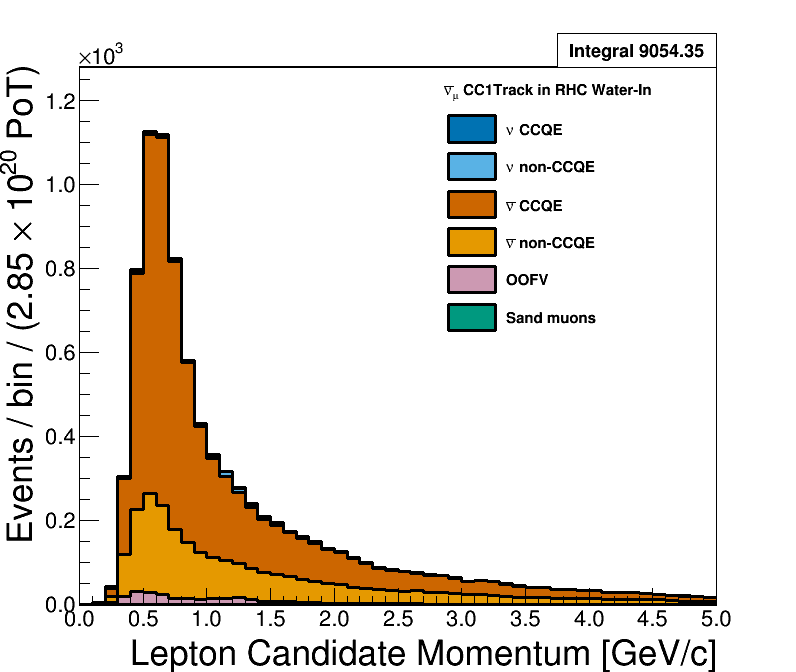
\includegraphics[width=0.45\textwidth]{Chapters/Figures/SamplesAndSelections/water/numubarRHC/CC1Track/FluxAndEventWeights/numubarRHCCC1TrackWaterIn_recoP_mu_MC_only_NEUTCCQELike_rhc_water}
\par\end{centering}
}\subfloat[$\cos\theta$]{\begin{centering}
`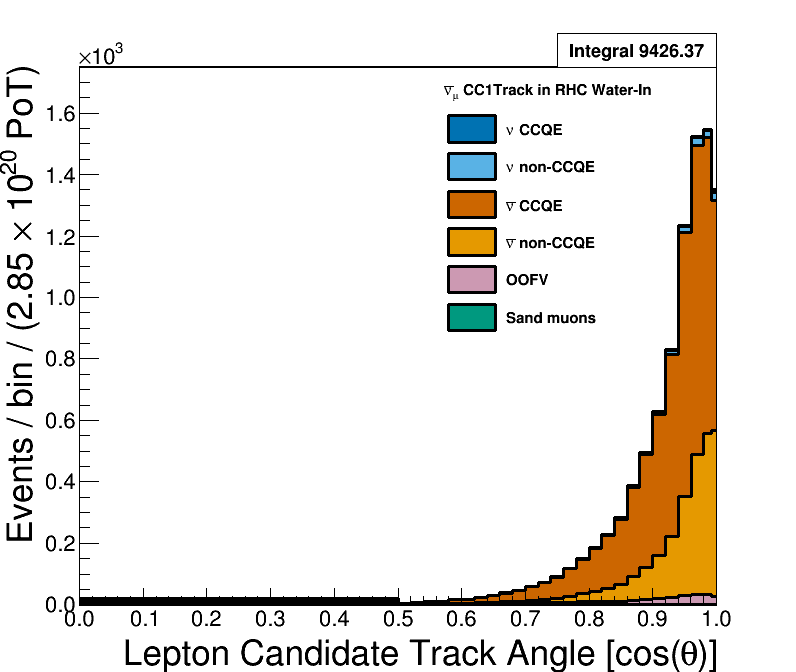
\includegraphics[width=0.45\textwidth]{Chapters/Figures/SamplesAndSelections/water/numubarRHC/CC1Track/FluxAndEventWeights/numubarRHCCC1TrackWaterIn_recocosq_mu_MC_only_NEUTCCQELike_rhc_water}
\par\end{centering}
}
\par\end{centering}
\caption[Reconstructed Kinematics of the $\numubar$ in RHC Mode CC 1-Track
Selection Categorized by CCQE and Non-CCQE Interactions]{Reconstructed kinematics of the $\protect\numubar$ in RHC Mode CC
1-Track selection categorized by CCQE and non-CCQE interactions. The
figures use the $\pod$ water-in MC and are normalized to the RHC
water-in mode POT. Also a single bin is used in the range of $0\protect\leq\cos\theta<0.5$
in figure (b).\label{fig:numubarRHCCC1TrkReco}}
\end{figure}

\begin{figure}
\begin{centering}
\subfloat[Water-in]{\begin{centering}
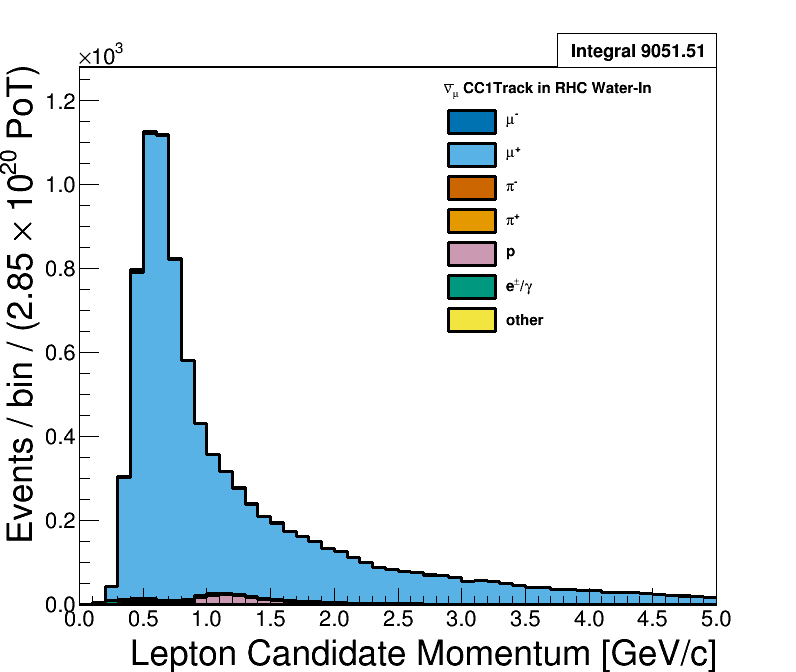
\includegraphics[width=0.45\textwidth]{Chapters/Figures/SamplesAndSelections/water/numubarRHC/CC1Track/FluxAndEventWeights/numubarRHCCC1TrackWaterIn_recoP_mu_MC_only_LeptonCandidateTruePDG_rhc_water}
\par\end{centering}
}\subfloat[Water-in]{\begin{centering}
`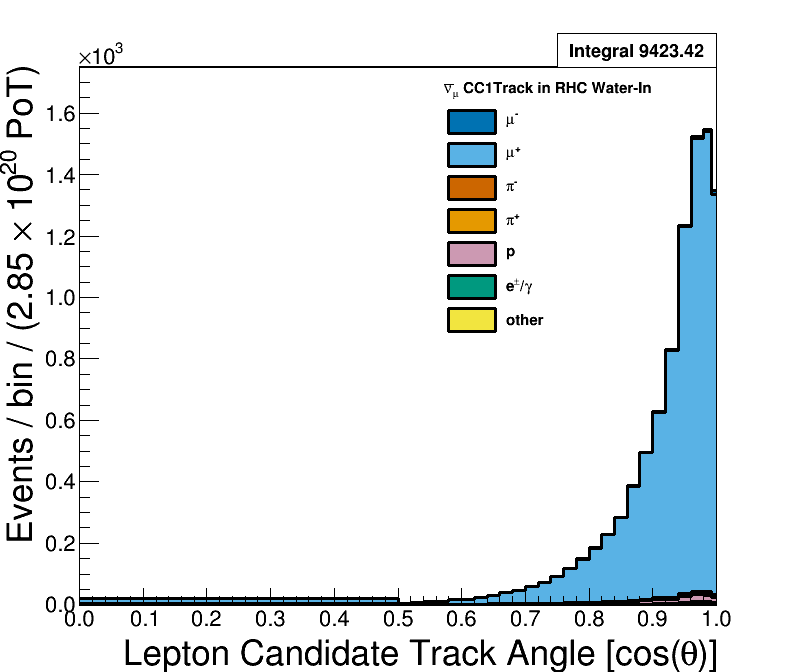
\includegraphics[width=0.45\textwidth]{Chapters/Figures/SamplesAndSelections/water/numubarRHC/CC1Track/FluxAndEventWeights/numubarRHCCC1TrackWaterIn_recocosq_mu_MC_only_LeptonCandidateTruePDG_rhc_water}
\par\end{centering}
}
\par\end{centering}
\caption[Reconstructed Kinematics of the $\numubar$ in RHC Mode CC 1-Track
Selection Categorized by the True Particle Matched to the Main Track]{Reconstructed kinematics of the $\protect\numubar$ in RHC Mode CC
1-Track selection categorized by the true particle matched to the
main track. The figures use the $\pod$ water-in MC and are normalized
to the RHC water-in mode POT. Also a single bin is used in the range
of $0\protect\leq\cos\theta<0.5$ in figure (b).\label{fig:numubarRHCCC1TrkRecoParticle}}
\end{figure}

We can examine the efficiencies and purities differentially for the
selection in \prettyref{fig:numubarRHCCC1TrkRecoEffPur}. For the
efficiency and purity only, the true signal is a true $\numubar$
CCQE interaction. The two distributions are very similar to the efficiency
and purity observed in the $\numu$ in FHC Mode CC 1-Track sample,
with the efficiency being relatively high (90\%) for high statistics
regions.

\begin{figure}
\begin{centering}
\subfloat[True $\protect\numubar$ CCQE Efficiency]{\begin{centering}
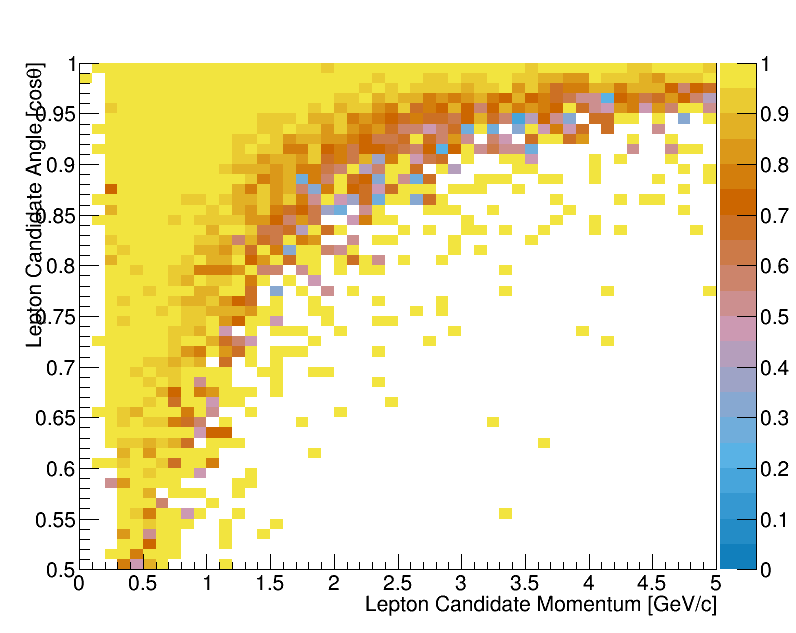
\includegraphics[width=0.45\textwidth]{Chapters/Figures/SamplesAndSelections/air/numubarRHC/CC1Track/FluxAndEventWeights/eff}
\par\end{centering}
}\subfloat[True $\protect\numubar$ CCQE Purity]{\begin{centering}
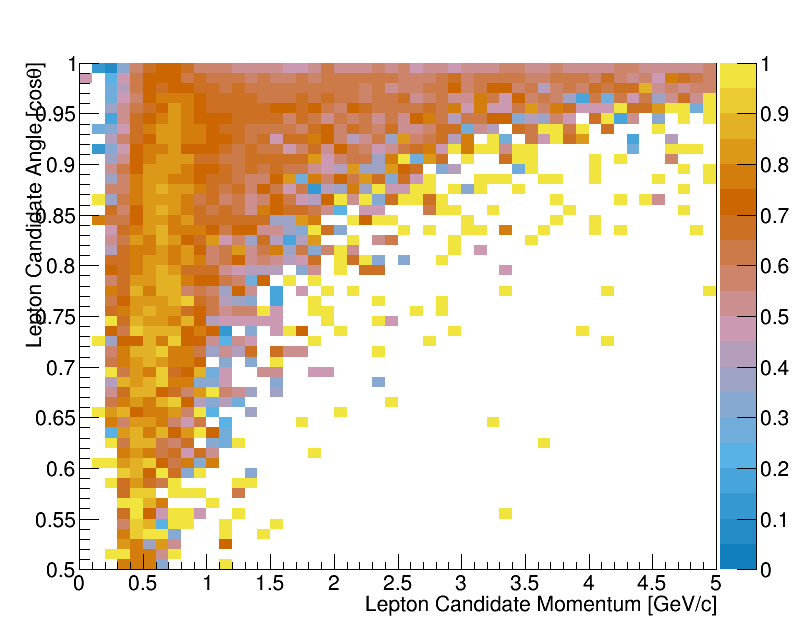
\includegraphics[width=0.45\textwidth]{Chapters/Figures/SamplesAndSelections/air/numubarRHC/CC1Track/FluxAndEventWeights/pur}
\par\end{centering}
}
\par\end{centering}
\caption[Efficiency and Purity of the $\numubar$ in RHC Mode CC 1-Track Selection]{Efficiency and purity of the $\protect\numubar$ in RHC Mode CC 1-Track
selection. The true events are $\protect\numubar$ CCQE at the vertex
and the selected lepton candidate is the true $\protect\muplus$.\label{fig:numubarRHCCC1TrkRecoEffPur}}
\end{figure}

The underlying true kinematics, $E_{\nu}$ and $Q^{2}$, of the interactions
are shown in \prettyref{fig:numubarRHCCC1TrkTrue}. We see a similar
true reaction composition with that of the $\numu$ in FHC Mode sample
in \mbox{Section~\ref{subsec:numuFHCCC1Trk}}. Most reactions are
true CCQE with a mixture of 2p2h and $1\pion$ events. As previously
seen in \mbox{Section~\ref{subsec:numuFHCCC1Trk}}, the significant
$1\pi$ contamination may reduce the sensitivity to both CC-$0\pi$
and CC-$1\pi$ model parameters in the BANFF fit.

\begin{figure}
\begin{centering}
\subfloat[True Neutrino Energy]{\begin{centering}
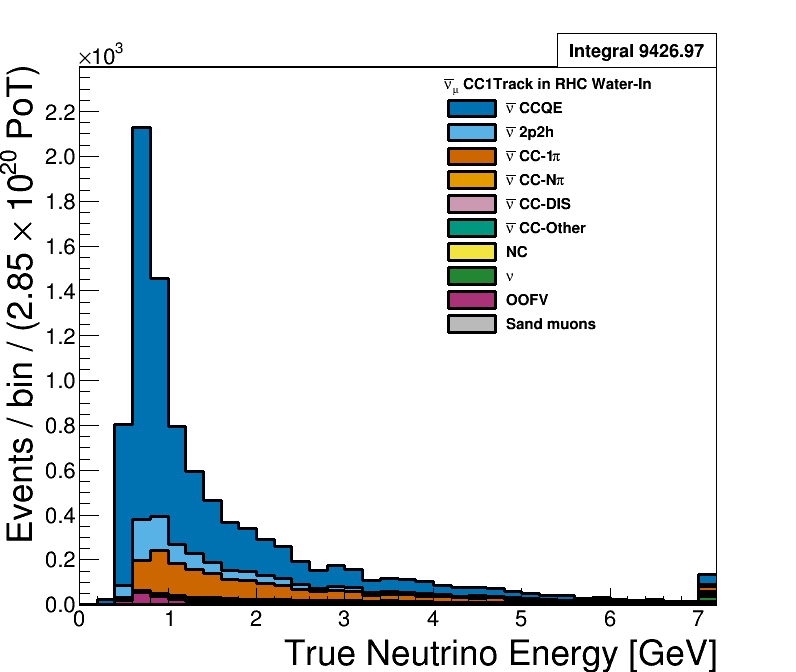
\includegraphics[width=0.45\textwidth]{Chapters/Figures/SamplesAndSelections/water/numubarRHC/CC1Track/FluxAndEventWeights/numubarRHCCC1TrackWaterIn_trueE_nu_MC_only_NEUTAntiNuReactionCodes_rhc_water}
\par\end{centering}
}\subfloat[True $Q^{2}$]{\begin{centering}
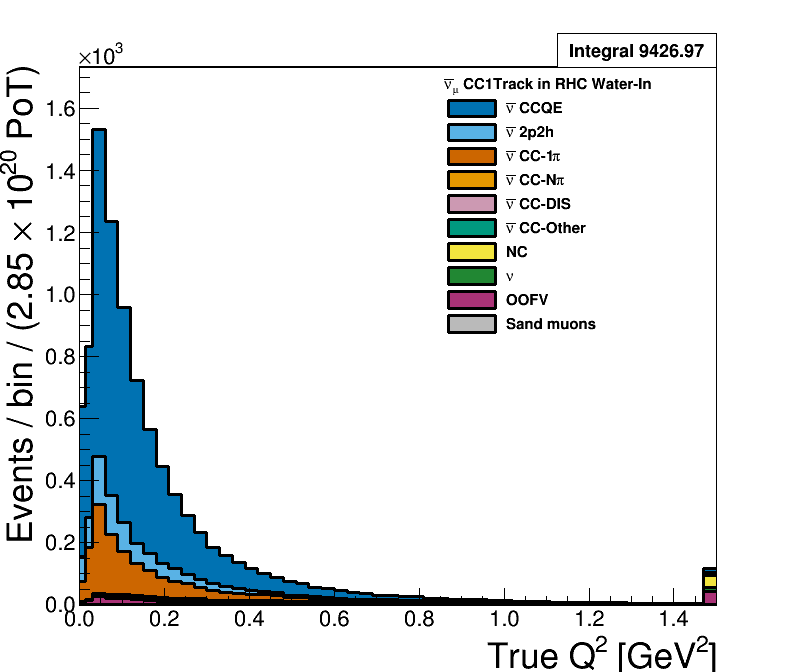
\includegraphics[width=0.45\textwidth]{Chapters/Figures/SamplesAndSelections/water/numubarRHC/CC1Track/FluxAndEventWeights/numubarRHCCC1TrackWaterIn_trueQ2_MC_only_NEUTAntiNuReactionCodes_rhc_water}
\par\end{centering}
}
\par\end{centering}
\caption[True Kinematics of the $\numubar$ in RHC Mode CC 1-Track Selection]{True kinematics of the $\protect\numubar$ in RHC Mode CC 1-Track
selection. Water-in mode is displayed here only with the last bin
shown is used as overflow. The figures use the $\pod$ water-in MC
and are normalized to the RHC water-in mode POT.\label{fig:numubarRHCCC1TrkTrue}}
\end{figure}


\subsection{The \numubartitle{} in RHC Mode CC N-Tracks Sample}

This selection provides the $\numubar$ non-CCQE-like samples in RHC
mode. \prettyref{fig:numubarRHCCCNTrkReco} and \prettyref{fig:numubarRHCCCNTrkRecoParticle}
display the momentum and angular distributions that are inputs to
BANFF. The most striking feature of this selection is the number of
mis-identified events. In particular tracks matched to protons are
selected as the HMPT when the protons are minimum ionizing particles
themselves, which is about $1.3$ GeV/c. In addition, the intrinsic
$\numu$ background contribution is comparable to the desired $\numubar$
flavor. These two features should be addressed to increase the utility
of the selection for the next iteration of the analysis.

\begin{figure}
\begin{centering}
\subfloat[Momentum]{\begin{centering}
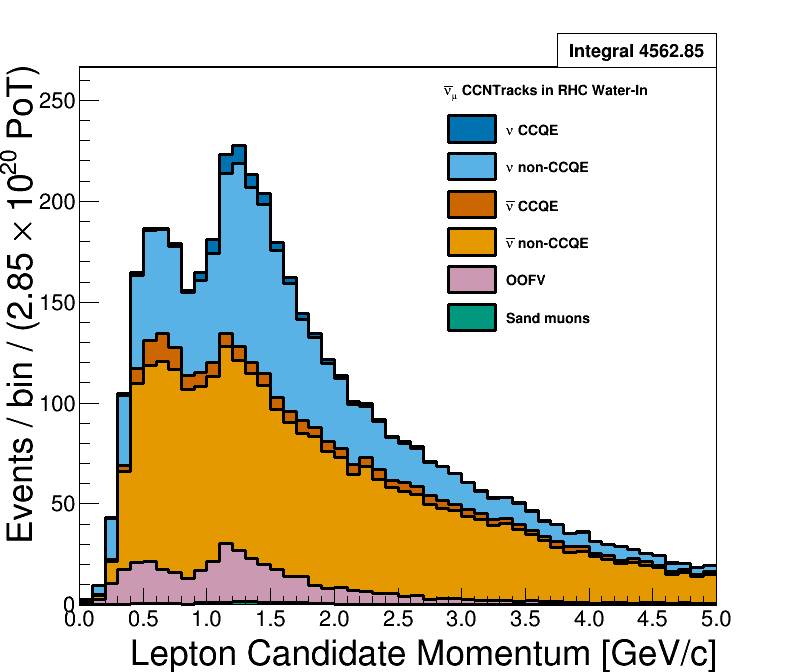
\includegraphics[width=0.45\textwidth]{Chapters/Figures/SamplesAndSelections/water/numubarRHC/CCNTracks/FluxAndEventWeights/numubarRHCCCNTracksWaterIn_recoP_mu_MC_only_NEUTCCQELike_rhc_water}
\par\end{centering}
}\subfloat[$\cos\theta$]{\begin{centering}
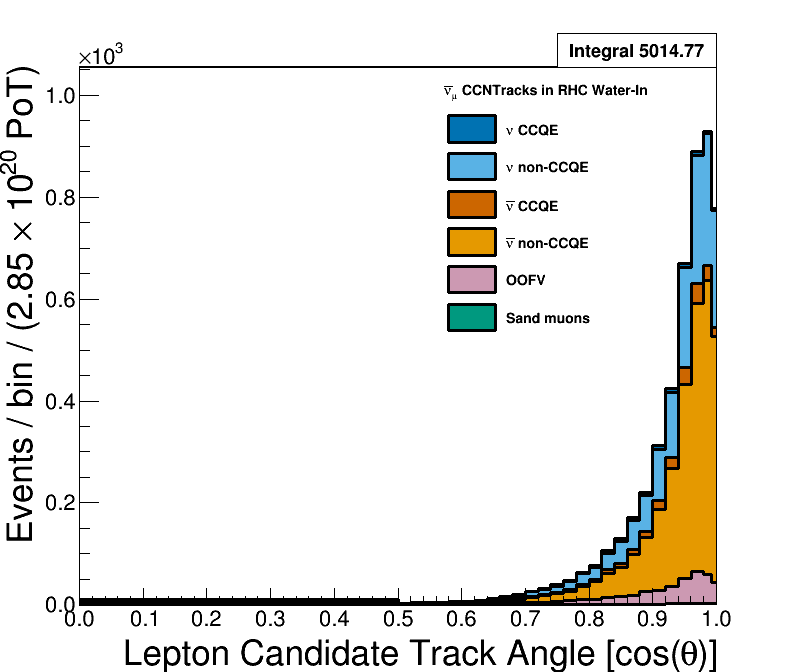
\includegraphics[width=0.45\textwidth]{Chapters/Figures/SamplesAndSelections/water/numubarRHC/CCNTracks/FluxAndEventWeights/numubarRHCCCNTracksWaterIn_recocosq_mu_MC_only_NEUTCCQELike_rhc_water}
\par\end{centering}
}
\par\end{centering}
\caption[Reconstructed Kinematics of the $\numubar$ in RHC Mode CC N-Tracks
Selection Categorized by CCQE and Non-CCQE Interactions]{Reconstructed kinematics of the $\protect\numubar$ in RHC Mode CC
N-Tracks selection categorized by CCQE and non-CCQE interactions.
The figures use the $\pod$ water-in MC and are normalized to the
RHC water-in mode POT. Also a single bin is used in the range of $0\protect\leq\cos\theta<0.5$
in figure (b).\label{fig:numubarRHCCCNTrkReco}}
\end{figure}

\begin{figure}
\begin{centering}
\subfloat[Momentum]{\begin{centering}
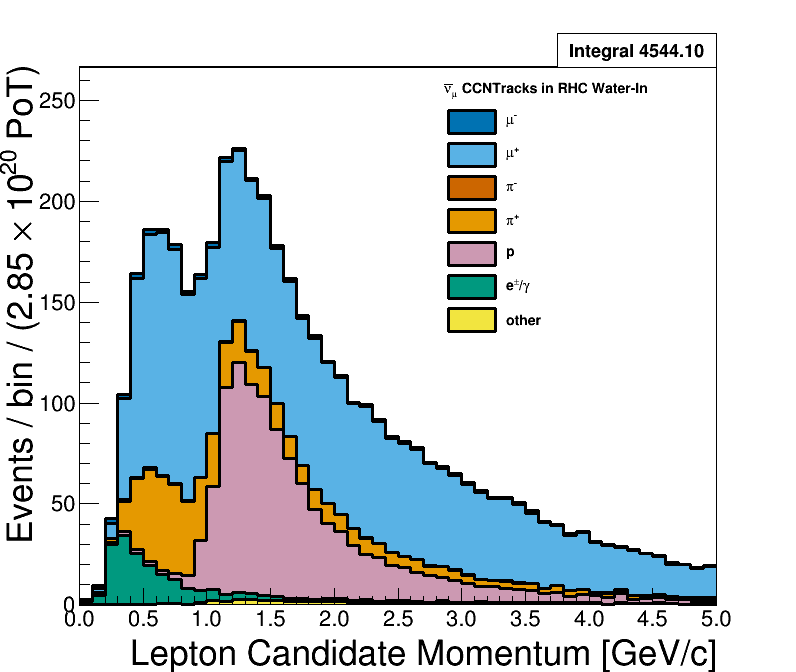
\includegraphics[width=0.45\textwidth]{Chapters/Figures/SamplesAndSelections/water/numubarRHC/CCNTracks/FluxAndEventWeights/numubarRHCCCNTracksWaterIn_recoP_mu_MC_only_LeptonCandidateTruePDG_rhc_water}
\par\end{centering}
}\subfloat[$\cos\theta$]{\begin{centering}
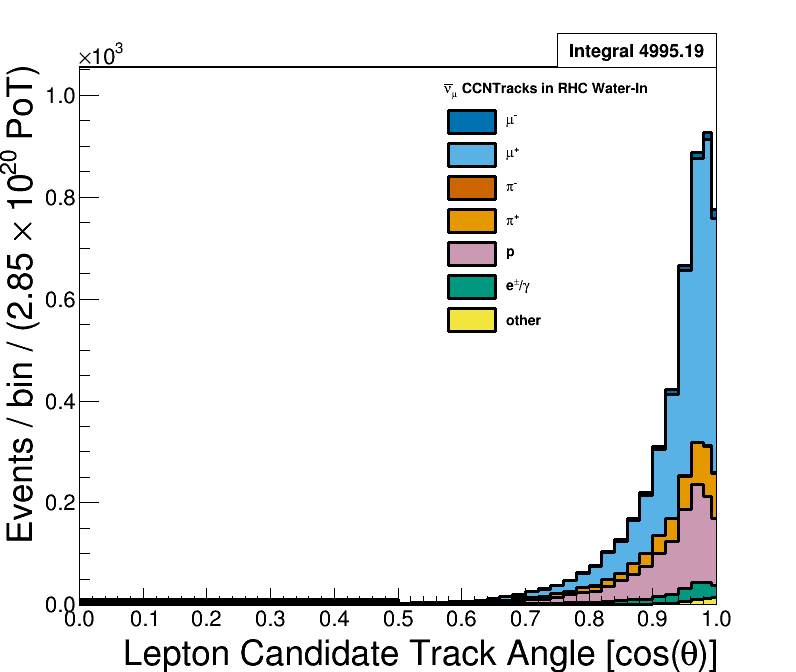
\includegraphics[width=0.45\textwidth]{Chapters/Figures/SamplesAndSelections/water/numubarRHC/CCNTracks/FluxAndEventWeights/numubarRHCCCNTracksWaterIn_recocosq_mu_MC_only_LeptonCandidateTruePDG_rhc_water}
\par\end{centering}
}
\par\end{centering}
\caption[Reconstructed Kinematics of the $\numubar$ in RHC Mode CC N-Tracks
Selection Categorized by the True Particle Matched to the Main Track]{Reconstructed kinematics of the $\protect\numubar$ in RHC Mode CC
N-Tracks selection categorized by the true particle matched to the
main track. The figures use the $\pod$ water-in MC and are normalized
to the RHC water-in mode POT. Also a single bin is used in the range
of $0\protect\leq\cos\theta<0.5$ in figure (b).\label{fig:numubarRHCCCNTrkRecoParticle}}
\end{figure}

We can examine the efficiencies and purities differentially for the
selection in \prettyref{fig:numuFHCCCNTrkRecoEffPur}. For the efficiency
and purity only, the true signal is any $\numubar$ CC interaction
except $\numubar$ CCQE which the CC 1-Track selection is designed
to select. Both the efficiency and purity are low where statistics
are high due to the wrong sign background.

\begin{figure}
\begin{centering}
\subfloat[True $\protect\numubar$ CC non-QE Efficiency]{\begin{centering}
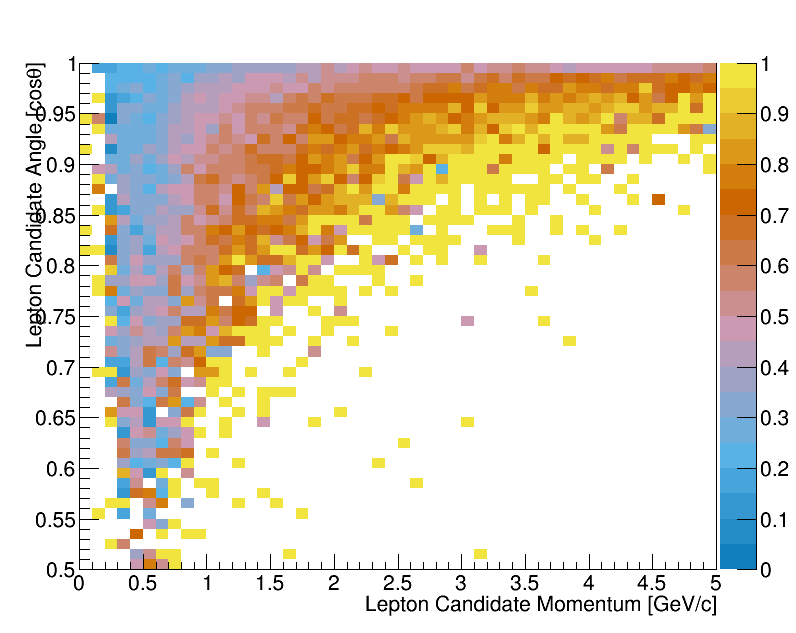
\includegraphics[width=0.45\textwidth]{Chapters/Figures/SamplesAndSelections/air/numubarRHC/CCNTracks/FluxAndEventWeights/eff}
\par\end{centering}
}\subfloat[True $\protect\numubar$ CC non-QE Purity]{\begin{centering}
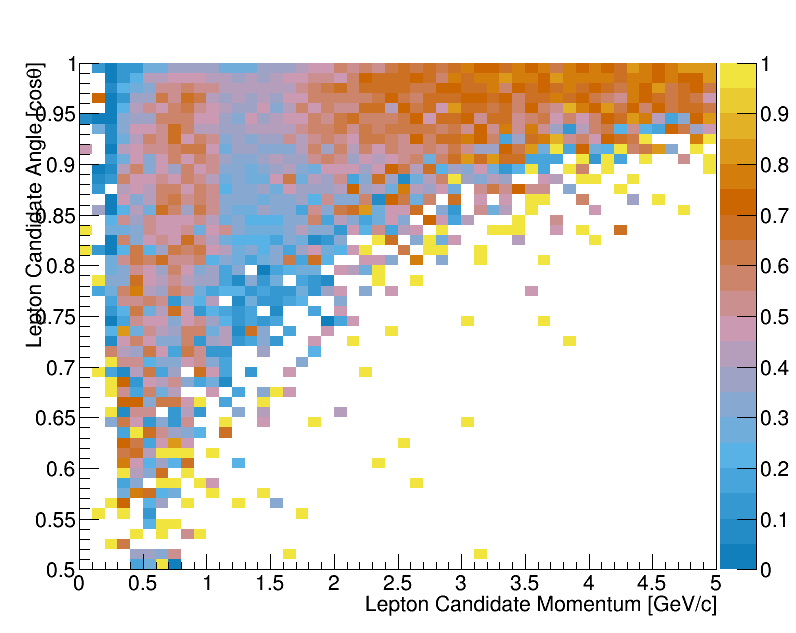
\includegraphics[width=0.45\textwidth]{Chapters/Figures/SamplesAndSelections/air/numubarRHC/CCNTracks/FluxAndEventWeights/pur}
\par\end{centering}
}
\par\end{centering}
\caption[Efficiency and Purity of the $\numubar$ in RHC Mode CC N-Tracks Selection]{Efficiency and purity of the $\protect\numubar$ in RHC Mode CC N-Tracks
selection. True events are defined as correctly matched $\protect\muplus$
tracks from $\protect\numubar$-induced CC non-QE interactions at
the vertex. \label{fig:numubarRHCCCNTrkRecoEffPur}}
\end{figure}

The underlying true kinematics, $E_{\nu}$, $Q^{2}$, and $W$, of
the interactions are shown in \prettyref{fig:numubarRHCCCNTrkTrue}.
Here we see in better detail the origin of the $\numu$ contamination.
As a function of increasing energy, the $\numubar$ content is decreasing
while the relative $\numu$ contribution is increasing. The $\numu$
events also have high $Q^{2}$ which explains the significant number
of misidentified proton main track events. For the hadronic final
states, the shape of the $\numubar$-induced resonances is similar
to what we saw in \prettyref{fig:numuFHCCCNTrkTrue}. Interestingly,
the $\numu$ background hadronic mass distribution does not peak in
any one region.

\begin{figure}
\begin{centering}
\subfloat[True Neutrino Energy]{\begin{centering}
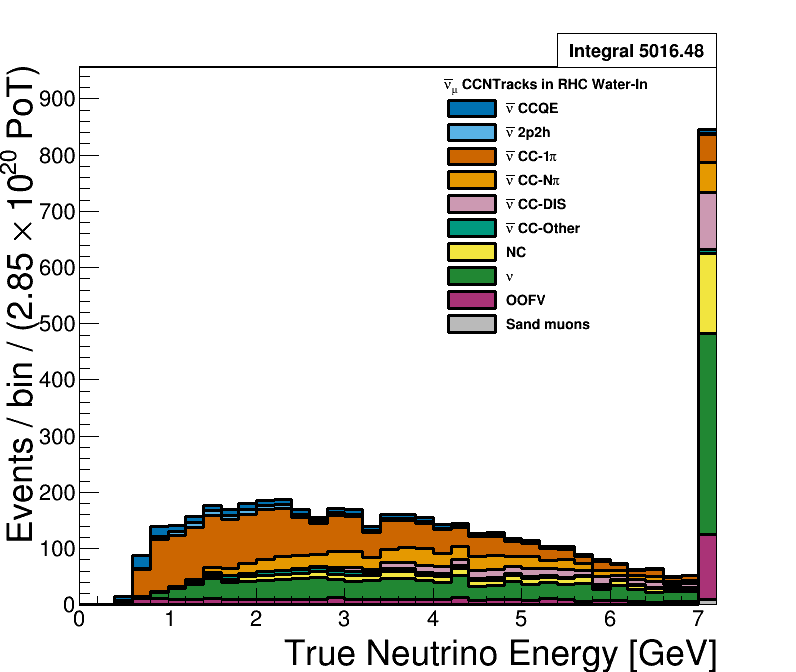
\includegraphics[width=0.45\textwidth]{Chapters/Figures/SamplesAndSelections/water/numubarRHC/CCNTracks/FluxAndEventWeights/numubarRHCCCNTracksWaterIn_trueE_nu_MC_only_NEUTAntiNuReactionCodes_rhc_water}
\par\end{centering}
}\subfloat[True $Q^{2}$]{\begin{centering}
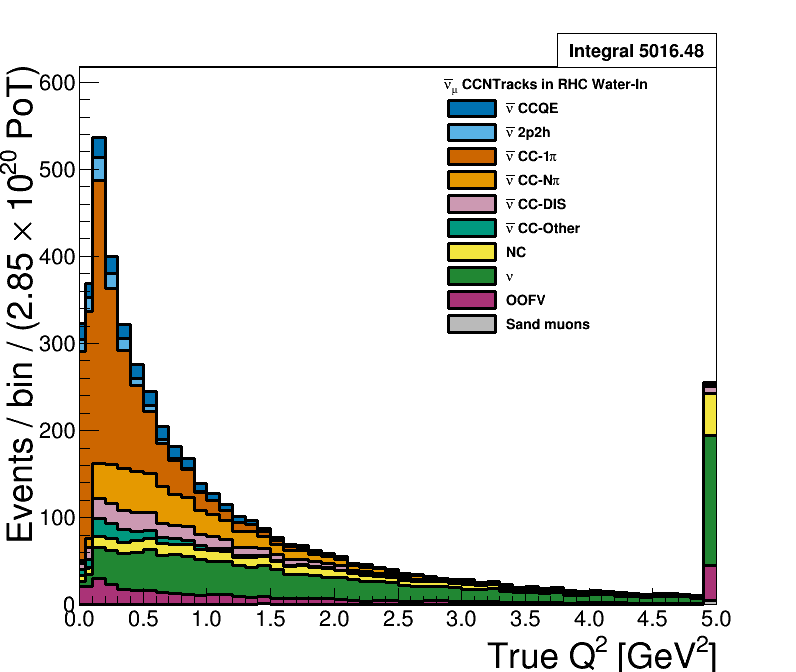
\includegraphics[width=0.45\textwidth]{Chapters/Figures/SamplesAndSelections/water/numubarRHC/CCNTracks/FluxAndEventWeights/numubarRHCCCNTracksWaterIn_trueQ2_MC_only_NEUTAntiNuReactionCodes_rhc_water}
\par\end{centering}
}
\par\end{centering}
\begin{centering}
\subfloat[True $W$]{\begin{centering}
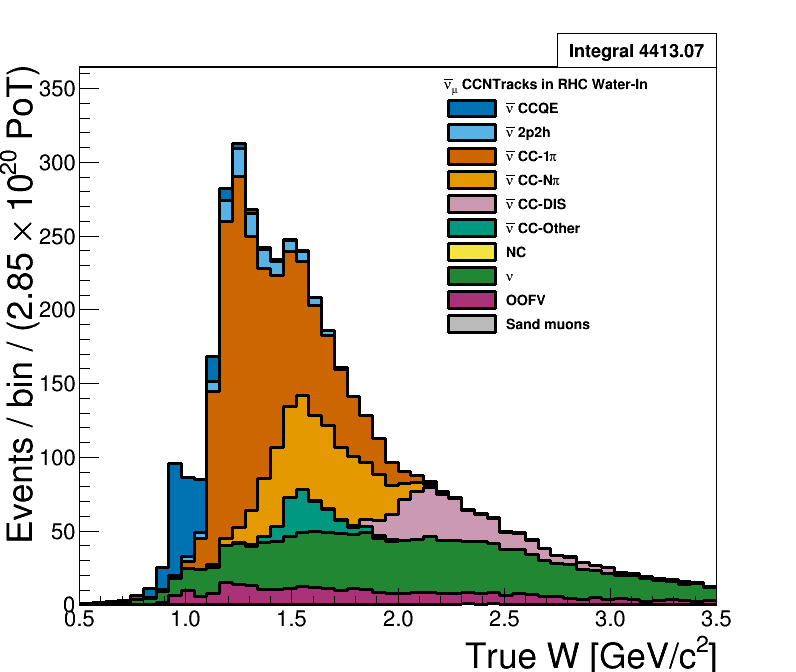
\includegraphics[width=0.45\textwidth]{Chapters/Figures/SamplesAndSelections/water/numubarRHC/CCNTracks/FluxAndEventWeights/numubarRHCCCNTracksWaterIn_trueW_MC_only_NEUTAntiNuReactionCodes_rhc_water}
\par\end{centering}
}
\par\end{centering}
\caption[True Kinematics of the $\numubar$ in RHC Mode CC N-Tracks Selection]{True kinematics of the $\protect\numubar$ in RHC Mode CC N-Tracks
selection. The last bin shown in (a) and (b) is used as overflow.
The figures use the $\pod$ water-in MC and are normalized to the
RHC water-in mode POT. \label{fig:numubarRHCCCNTrkTrue}}
\end{figure}


\subsection{The \numutitle{} Background in RHC Mode CC 1-Track Sample}

This selection provides the $\numu$ in RHC, also called wrong-sign
background, CCQE-like samples . \prettyref{fig:numuRHCCC1TrkReco}
and \prettyref{fig:numuRHCCC1TrkRecoParticle} display the momentum
and angular distributions inputs to the BANFF fit. We can see this
is a relatively low-angle selection compared to previous selections.
Importantly the selection is relatively $\numu$-pure which should
help constrain the wrong-sign background in the fit. However, the
CCQE purity is modest given number of correctly identified lepton
candidates. This feature needs to be addressed in the next iteration
of the analysis.

\begin{figure}
\begin{centering}
\subfloat[Momentum]{\begin{centering}
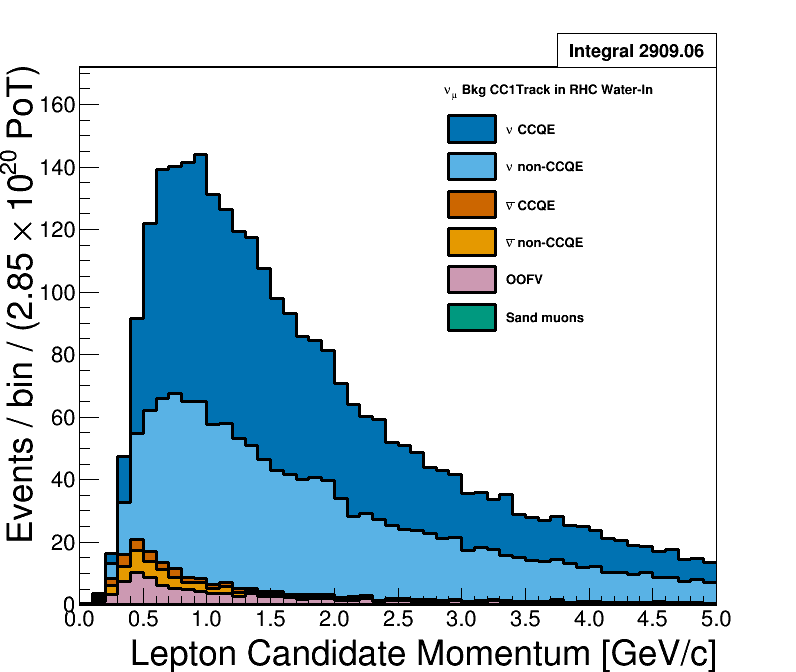
\includegraphics[width=0.45\textwidth]{Chapters/Figures/SamplesAndSelections/water/numubkgRHC/CC1Track/FluxAndEventWeights/numubkgRHCCC1TrackWaterIn_recoP_mu_MC_only_NEUTCCQELike_rhc_water}
\par\end{centering}
}\subfloat[$\cos\theta$]{\begin{centering}
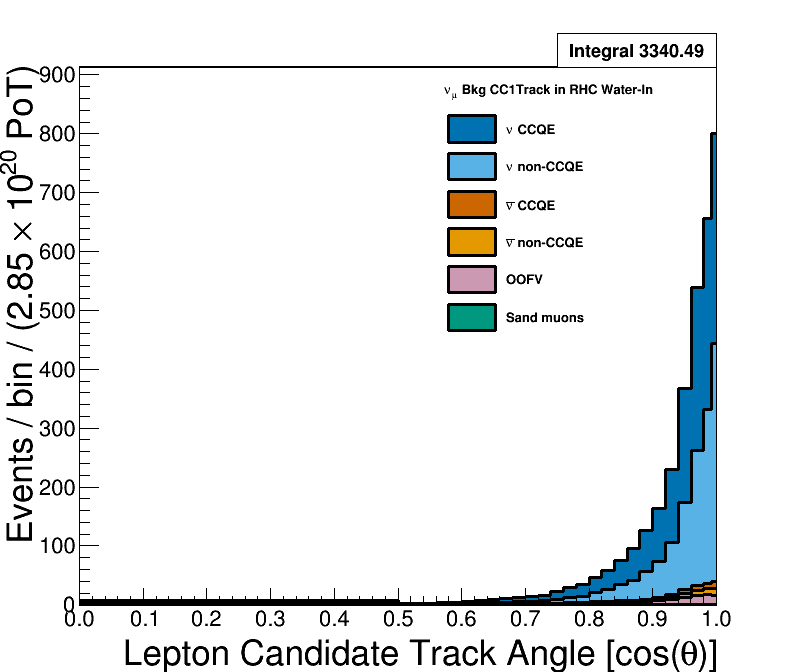
\includegraphics[width=0.45\textwidth]{Chapters/Figures/SamplesAndSelections/water/numubkgRHC/CC1Track/FluxAndEventWeights/numubkgRHCCC1TrackWaterIn_recocosq_mu_MC_only_NEUTCCQELike_rhc_water}
\par\end{centering}
}
\par\end{centering}
\caption[Reconstructed Kinematics of the $\numu$ Background in RHC Mode CC
1-Track Selection Categorized by CCQE and Non-CCQE Interactions]{Reconstructed kinematics of the $\protect\numu$ Background in RHC
Mode CC 1-Track selection categorized by CCQE and non-CCQE interactions.
The figures use the $\pod$ water-in MC and are normalized to the
RHC water-in mode POT. Also a single bin is used in the range of $0\protect\leq\cos\theta<0.5$
in figure (b).\label{fig:numuRHCCC1TrkReco}}
\end{figure}

\begin{figure}
\begin{centering}
\subfloat[Momentum]{\begin{centering}
\includegraphics[width=0.45\textwidth]{Chapters/Figures/SamplesAndSelections/water/numubkgRHC/CC1Track/FluxAndEventWeights/numubkgRHCCC1TrackWaterIn_recoP_mu_MC_only_LeptonCandidateTruePDG_rhc_water}
\par\end{centering}
}\subfloat[$\cos\theta$]{\begin{centering}
\includegraphics[width=0.45\textwidth]{Chapters/Figures/SamplesAndSelections/water/numubkgRHC/CC1Track/FluxAndEventWeights/numubkgRHCCC1TrackWaterIn_recocosq_mu_MC_only_LeptonCandidateTruePDG_rhc_water}
\par\end{centering}
}
\par\end{centering}
\caption[Reconstructed Kinematics of the $\numu$ Background in RHC Mode CC
1-Track Selection Categorized by the True Particle Matched to the
Main Track]{Reconstructed kinematics of the $\protect\numu$ Background in RHC
Mode CC 1-Track selection categorized by the true particle matched
to the main track. The figures use the $\pod$ water-in MC and are
normalized to the RHC water-in mode POT. Also a single bin is used
in the range of $0\protect\leq\cos\theta<0.5$ in figure (b).\label{fig:numuRHCCC1TrkRecoParticle}}
\end{figure}

We can examine the efficiencies and purities differentially for the
selection in \prettyref{fig:numuRHCCC1TrkRecoEffPur}. For the efficiency
and purity only, the true signal is a true $\numu$ CCQE interaction.
The efficiency is similar to the $\numu$ in FHC Mode CC 1-Track topology
efficiency with banded $p-\theta$ regions. As for the purity, it
is roughly 70\% in a banded region between low momenta, low angle
and high momenta, high angle tracks.

\begin{figure}
\begin{centering}
\subfloat[True $\protect\numu$ CCQE Efficiency]{\begin{centering}
\includegraphics[width=0.45\textwidth]{Chapters/Figures/SamplesAndSelections/air/numubkgRHC/CC1Track/FluxAndEventWeights/eff}
\par\end{centering}
}\subfloat[True $\protect\numu$ CCQE Purity]{\begin{centering}
\includegraphics[width=0.45\textwidth]{Chapters/Figures/SamplesAndSelections/air/numubkgRHC/CC1Track/FluxAndEventWeights/pur}
\par\end{centering}
}
\par\end{centering}
\caption[Efficiency and Purity of the $\numu$ Background in RHC Mode CC 1-Track
Selection]{Efficiency and purity of the $\protect\numu$ Background in RHC Mode
CC 1-Track selection. The true events are $\protect\numu$ CCQE at
the vertex and the selected lepton candidate is the true $\protect\muminus$.
\label{fig:numuRHCCC1TrkRecoEffPur}}
\end{figure}

The underlying true kinematics, $E_{\nu}$ and $Q^{2}$, of the selection
are shown in \prettyref{fig:numuRHCCC1TrkTrue}. The number of the
wrong-sign background events peaks at 1 GeV and is a broad peak compared
to the designed sharp $\numubar$ peak at 0.6 GeV as shown in \prettyref{fig:numubarRHCCC1TrkTrue}.
Since these are higher energy events, there is more available energy
to produce resonance states that produce $1\pi$ topologies. This
explains the significant non-CCQE event contamination.

\begin{figure}
\begin{centering}
\subfloat[True Neutrino Energy]{\begin{centering}
\includegraphics[width=0.45\textwidth]{Chapters/Figures/SamplesAndSelections/water/numubkgRHC/CC1Track/FluxAndEventWeights/numubkgRHCCC1TrackWaterIn_trueE_nu_MC_only_NEUTNuReactionCodes_rhc_water}
\par\end{centering}
}\subfloat[True $Q^{2}$]{\begin{centering}
\includegraphics[width=0.45\textwidth]{Chapters/Figures/SamplesAndSelections/water/numubkgRHC/CC1Track/FluxAndEventWeights/numubkgRHCCC1TrackWaterIn_trueQ2_MC_only_NEUTNuReactionCodes_rhc_water}
\par\end{centering}
}
\par\end{centering}
\caption[True Kinematics of the $\numu$ Background in RHC Mode CC 1-Track
Selection]{True kinematics of the $\protect\numu$ Background in RHC Mode CC
1-Track selection. Water-in mode is displayed here only with the last
bin shown is used as overflow. The figures use the $\pod$ water-in
MC and are normalized to the RHC water-in mode POT.\label{fig:numuRHCCC1TrkTrue}}
\end{figure}


\subsection{The \numutitle{} Background in RHC Mode CC N-Tracks Sample}

This selection provides the non-CCQE-like samples for the $\numu$
background in RHC mode. \prettyref{fig:numuRHCCCNTrkReco} and \prettyref{fig:numuRHCCCNTrkRecoParticle}
show the momentum and angular distributions that are inputs to the
BANFF fit. We can see the selection is relatively $\numu$-pure with
a significant mis-identified track rate. Interestingly, the misidentified
pion main tracks have a high momentum tail.

\begin{figure}
\begin{centering}
\subfloat[Momentum]{\begin{centering}
\includegraphics[width=0.45\textwidth]{Chapters/Figures/SamplesAndSelections/water/numubkgRHC/CCNTracks/FluxAndEventWeights/numubkgRHCCCNTracksWaterIn_recoP_mu_MC_only_NEUTCCQELike_rhc_water}
\par\end{centering}
}\subfloat[$\cos\theta$]{\begin{centering}
\includegraphics[width=0.45\textwidth]{Chapters/Figures/SamplesAndSelections/water/numubkgRHC/CCNTracks/FluxAndEventWeights/numubkgRHCCCNTracksWaterIn_recocosq_mu_MC_only_NEUTCCQELike_rhc_water}
\par\end{centering}
}
\par\end{centering}
\caption[Reconstructed Kinematics of the $\numu$ Background in RHC Mode CC
N-Tracks Selection Categorized by CCQE and Non-CCQE Interactions]{Reconstructed kinematics of the $\protect\numu$ Background in RHC
Mode CC 1-Track selection categorized by CCQE and non-CCQE interactions.
The figures use the $\pod$ water-in MC and are normalized to the
RHC water-in mode POT. Also a single bin is used in the range of $0\protect\leq\cos\theta<0.5$
in figure (b).\label{fig:numuRHCCCNTrkReco}}
\end{figure}

\begin{figure}
\begin{centering}
\subfloat[Momentum]{\begin{centering}
\includegraphics[width=0.45\textwidth]{Chapters/Figures/SamplesAndSelections/water/numubkgRHC/CCNTracks/FluxAndEventWeights/numubkgRHCCCNTracksWaterIn_recoP_mu_MC_only_LeptonCandidateTruePDG_rhc_water}
\par\end{centering}
}\subfloat[$\cos\theta$]{\begin{centering}
\includegraphics[width=0.45\textwidth]{Chapters/Figures/SamplesAndSelections/water/numubkgRHC/CCNTracks/FluxAndEventWeights/numubkgRHCCCNTracksWaterIn_recocosq_mu_MC_only_LeptonCandidateTruePDG_rhc_water}
\par\end{centering}
}
\par\end{centering}
\caption[Reconstructed Kinematics of the $\numu$ Background in RHC Mode CC
N-Tracks Selection Categorized by the True Particle Matched to the
Main Track]{Reconstructed kinematics of the $\protect\numu$ Background in RHC
Mode CC 1-Track selection categorized by the true particle matched
to the main track. The figures use the $\pod$ water-in MC and are
normalized to the RHC water-in mode POT. Also a single bin is used
in the range of $0\protect\leq\cos\theta<0.5$ in figure (b).\label{fig:numuRHCCCNTrkRecoParticle}}
\end{figure}

We can examine the $\numu$ CC non-QE efficiency and purity of the
selection in \prettyref{fig:numuRHCCCNTrkRecoEffPur}. There is a
reduction in the purity below 1.5 GeV/c due to the the $\numubar$
selections occupying the same phase space. Fortunately, the efficiency
and purity are relatively high above 1.5 GeV/c.

\begin{figure}
\begin{centering}
\subfloat[True $\protect\numu$ CC non-QE Efficiency]{\begin{centering}
\includegraphics[width=0.45\textwidth]{/home/mhogan/Documents/graduateDisseration/Chapters/Figures/SamplesAndSelections/air/numubkgRHC/CCNTracks/FluxAndEventWeights/eff}
\par\end{centering}
}\subfloat[True $\protect\numu$ CC non-QE Purity]{\begin{centering}
\includegraphics[width=0.45\textwidth]{/home/mhogan/Documents/graduateDisseration/Chapters/Figures/SamplesAndSelections/air/numubkgRHC/CCNTracks/FluxAndEventWeights/pur}
\par\end{centering}
}
\par\end{centering}
\caption[Efficiency and Purity of the $\numu$ Background in RHC Mode CC N-Tracks
Selection]{Efficiency and purity of the $\protect\numu$ Background in RHC Mode
CC N-Tracks selection. True events are defined as correctly matched
$\protect\muminus$ tracks from $\protect\numu$-induced CC non-QE
interactions at the vertex. \label{fig:numuRHCCCNTrkRecoEffPur}}
\end{figure}

The underlying true kinematics, $E_{\nu}$, $Q^{2}$, and $W$, of
the interactions are shown in \prettyref{fig:numuRHCCCNTrkTrue}.
As we have seen before with the CC N-Tracks samples, these are high
$E_{\nu}$ events with large $Q^{2}$ exchanges. The invariant hadronic
system displays the previously seen resonances, with the largest still
being from the $\Delta$ baryon.

\begin{figure}
\begin{centering}
\subfloat[True Neutrino Energy]{\begin{centering}
\includegraphics[width=0.45\textwidth]{Chapters/Figures/SamplesAndSelections/water/numubkgRHC/CCNTracks/FluxAndEventWeights/numubkgRHCCCNTracksWaterIn_trueE_nu_MC_only_NEUTNuReactionCodes_rhc_water}
\par\end{centering}
}\subfloat[True $Q^{2}$]{\begin{centering}
\includegraphics[width=0.45\textwidth]{Chapters/Figures/SamplesAndSelections/water/numubkgRHC/CCNTracks/FluxAndEventWeights/numubkgRHCCCNTracksWaterIn_trueQ2_MC_only_NEUTNuReactionCodes_rhc_water}
\par\end{centering}
}
\par\end{centering}
\begin{centering}
\subfloat[True $W$]{\begin{centering}
\includegraphics[width=0.45\textwidth]{Chapters/Figures/SamplesAndSelections/water/numubkgRHC/CCNTracks/FluxAndEventWeights/numubkgRHCCCNTracksWaterIn_trueW_MC_only_NEUTNuReactionCodes_rhc_water}
\par\end{centering}
}
\par\end{centering}
\caption[True Kinematics of the $\numu$ Background in RHC Mode CC N-Tracks
Selection]{True kinematics of the $\protect\numu$ Background in RHC Mode CC
N-Tracks selection. The last bin shown in (a) and (b) is used as overflow.
The figures use the $\pod$ water-in MC and are normalized to the
RHC water-in mode POT. \label{fig:numuRHCCCNTrkTrue}}
\end{figure}


\section{Summary\label{sec:SelectionSummary}}

In this chapter we have examined the selection true and reconstruction
kinematics that will used in the BANFF fit. We see the 1-Track selections
yield some reasonably pure CCQE samples. By inverting that cut, we
obtain some information on the rate of other topologies like CC-$1\pi$
and high $Q^{2}$ CCDIS events. Importantly is the ability of these
samples to constrain the correct sign ($\numubar$) and wrong sign
($\numu$) backgrounds in RHC mode, which are very important in the
oscillation analysis. We can now move forward to the next chapter
to describe the fit parameters and the systematic uncertainties present
in the analysis.
